\chapter{State of the Art}\label{chapter:sota}
This chapter presents the state of the art (SotA) regarding approaches for GDPR compliance.
The first section (\autoref{sec:sota:models}) presents an overview of technological approaches for legal compliance to date.
The second section (\autoref{sec:sota:gdpr-semweb}) presents an overview of approaches for GDPR compliance utilising semantic web, with the third section (\autoref{sec:sota:gdpr-other}) presenting other approaches for GDPR compliance,
while the fourth section (\autoref{sec:sota:other}) presents approaches regarding regulatory compliance which do not directly concern the GDPR but are relevant towards understanding the SotA.
The chapter concludes (\autoref{sec:sota:analysis}) with an analysis of presented approaches and a discussion on the identified gaps for further work in the domain of utilising semantic web for GDPR compliance.

\section{Overview of Technological Approaches for Legal Compliance}\label{sec:sota:models}
This section provides an overview of technological approaches utilised for addressing legal compliance. It presents the different methodologies and frameworks for interpreting requirements from legal documents, and using technological frameworks towards the management of information and compliance.
To that end, the section utilises surveys and key publications in the last decade (2007-2019) to identify the state of the art.

\subsection{Classification of Approaches}
% 1> surveys of high level approaches to legal compliance
A survey of approaches within the last 50 years (from 2007) for addressing legal requirements \cite{otto_addressing_2007} provides the following categorisation:
\begin{itemize}
    \item \textbf{symbolic or mathematical logic}:  This approach attempts to balance use of natural language in legal documents with symbolic logic in an attempt to avoid ambiguities in interpretation. One of the earliest approaches, it was the precursor to later representations for machine and human readability.
    \item \textbf{knowledge representation}: This approach attempts to represent legal text as computer programs or algorithms by using logic programming techniques, primarily using Prolog, to avoid ambiguities in interpretation. The approach has been applied only within rigid domains where the law has minimal changes and does not rely on case law for interpretation. Additionally, the approach requires manual construction of logic rules from legal text, which prevents traceability. These challenges have limited its application to areas requiring requirements for system design, such as in software.
	\item \textbf{deontic logic}: This is another logic-based approach which involves capturing the rights and obligations provided within the law. The approach can be extending from representing this information to utilising it for preparing and assessing of compliance. This provides the necessary requirements which can be utilised in the development of business processes for legal compliance. Deontic logic has also been utilised to represent licensing and agreement requirements similar to those as legal text \cite{pellegrini_genealogy_2018}, and continues to be a topic of research in the areas of legal compliance \cite{palmirani_pronto:_2018,agarwal_legislative_2018,vos_odrl_2019}.
	\item \textbf{defeasible logic}: This approach consists of formulating rules of different types, namely - strict rules, defeasible rules, and defeaters - in order to represent the normative requirements extracted from legal text. Within the approach, strict rules must always hold, while defeasible rules hole true unless countered by an exception of a defeater. The approach is promised to provide better representation of conflicts in legal text in terms of interpretation as well as governance and jurisdiction requirements.
	\item \textbf{first order temporal logic}: This approach is based on using first-order temporal logic to extract key concepts such as - context, roles, type of information - and constructing logic-based requirements from those. The approach has not seen a large amount of interest, with existing applications limited to the privacy domain, and utilised for assessing compliance between privacy policies and laws.
	\item \textbf{access control }: Access control techniques have been utilised to capture the privacy-related elements of legal texts in the form of conditions and obligations that must be incorporated into a system as normative requirements for access to information. Conditions and obligations that cannot be represented as access control rules are incorporated as external environmental flags within the requirements. Utilising access control provides compliance by design, with logging providing transparency and accountability in the process. A survey of access control approaches utilising semantic web \cite{kirrane_access_2016} provides an overview of its applicability for different domains, including privacy enforcement.
	\item \textbf{markup-based representations}: This approach involves representing the hierarchical structure of legal text using markup-based representations such as SGML and XML. The representation enables the annotation of legal text and addition of metadata pertaining to definitions, acronyms, and citations. It also enables associating information about compliance requirements as well as interpretation. The United Nations and European Commission utilise this approach in publication of legislations and case law through standardised ontologies  \cite{palmirani_akoma_2018,european_union_eli_2015,van_opijnen_european_2011}.
	\item \textbf{goal based modelling}: This approach involves extracting and representing goals, soft goals, tasks, resources, and social relationships and modelling obligations to represent relationships for actors, dependencies, trust, delegation, and goal refinement. 
	\item \textbf{reusable requirements catalogue}: This approach constructs reusable catalogue of legal requirements derived from legal texts which are then applied to development lifecycles to incorporate compliance into systems. The use of the catalogue enables uncovering ambiguities and inconsistencies through use, and the refinement of the approach over time. The approach has been applied regarding security and personal data protection.
\end{itemize}

The survey paper provides comments on the applicability as well as limitation of each approach, and  outlines the following requirements engineering objectives (prefix \textit{REO}) an approach must take with in legal contexts to support the analysis of regulatory texts for requirements specification, system design, and compliance monitoring:
\begin{enumerate}[label={\textit{REO.\theenumi}}]
    \item \textbf{Identification of relevant regulations}: Finding relevant laws for a given system or process requires understanding of both - the requirements of the process as well as the context of the law. In addition, incorporating case law provides further challenges regarding application of relevant laws to processes due to the specifics and interpretation of requirements involved.
    \item \textbf{Classification of regulations with metadata}: In view of the above, the regulations need to be annotated or associated with metadata which can be utilised to classify them. This has been achieved to some extent through the EuroVoc\footnote{\url{https://eur-lex.europa.eu/browse/eurovoc.html}} - which is used as a multilingual and multidisciplinary thesaurus in the publication of metadata associated with EU legislations. However, where EuroVoc provides metadata about the domain of the legislation, greater granularity is needed to identify relevant information such as concepts, use-cases, and roles within the legal text.
    \item \textbf{Prioritisation of regulations and exceptions}: The hierarchical structure of regulations as well as relation to other regulations in terms of exceptions as well as overlaps and contradictions  must be taken into account for developing requirements.
    \item \textbf{Management of evolving regulations and law}: Changes in regulations need to be assessed by comparing the regulations, understanding the changes in requirements, and their application to existing systems for compliance. This requires traceability between legislations and requirements.
    \item \textbf{Traceability between references and requirements}: From the above, it is necessary to provide traceability from any section or clause with a reference in the legislation to the legal text being referenced. This is required in order to enable understanding of derived requirements from such sections across legislations.
    \item \textbf{Data Dictionary and glossary to ensure consistency}: Regulatory compliance makes use of consistent definitions and terminology an important aspect of requirements engineering. These are represented in the form of a data dictionary for domain-specific definitions and acronyms, and are utilised to support the requirements engineering process in providing a unified glossary for specifications, design, and compliance. 
    \item \textbf{Semi-automated navigation and searching}: The legislation needs to be accessible in both machine-readable as well as human-understandable states so as to enable technological approaches such as information extraction, annotations, searching, and automation in traceability of related information.
    \item \textbf{Annotation of regulatory statements}: It must be possible to associate annotations or additional information to regulatory statements, for example, with clarification of ambiguities or relevant case laws. Additionally, such annotations are also useful in a requirements engineering process to record assumptions and interpretations, and their usage in systems and applications.
    \item \textbf{Queries comparing legal concepts and compliance}: Finally, it must be possible query for information both within the text of the regulation as well as its associated information in order to support disambiguation and auditing for compliance. 
    Queries can assist with identification and comparison of applicable regulations, and to assess whether a particular requirement derived from the regulation has been addressed with respect to its compliance.
\end{enumerate}

\subsubsection{Discussion}
While the survey paper does not explicitly mention or refer to the linked data principles \cite{bizer_linked_2011}, some of the above objectives are fulfilled by utilising them in a given approach. Namely, linked data and semantic web provide an interoperable representation based in standards which can be used to define the required metadata regarding legislations, as demonstrated by EuroVoc, which addresses \textit{REO.1}, \textit{REO.2}, and \textit{REO.6} to some extent.

The use of structured representation to define legislations for \textit{REO.3} and \textit{REO.7} is possible using XML and ontologies such as ELI and Akoma Ntoso. However, ELI does not currently offer a way to represent the hierarchical structure of regulations, such as representation of individual articles or clauses, though the European Commission's Publication Office has stated their intention to provide this feature in the future.
This also limits the applications of \textit{REO.4} and \textit{REO.5} which require the above representation.
For creation of glossaries from legal text, the requirements of \textit{REO.6} are addressed through existing efforts such as EuroVoc and Interactive Terminology for Europe\footnote{\url{https://iate.europa.eu/}} (IATE), which provide consistent use of terms across domains, though there are no mechanisms to derive definitions from legislations or common interpretations of terms.

Regarding annotations for \textit{REO.8}, there exist standards such as W3C's Web Annotations model\footnote{\url{https://www.w3.org/annotation/}}, which can be utilised to annotate documents in an interoperable format, though they are not intended nor directly applicable for use over legislations.
Limitations to this are a lack of structured representation with sufficient granularity, for example, to reference individual clauses of text within the document.
Querying, as required for \textit{REO.9}, is inherently dependant on the underlying information representation, though there are standards such as SQL and SPARQL which provide interoperability in the approach.

\subsection{Approaches based on business process representations}
The use of approaches utilising business process representations for compliance are summarised in two key surveys. The first \cite{fellmann_state---art_2014} relates to the use of business processes within different phases of compliance, while the second \cite{benyoucef_information_2015} analyses use of information artefacts in business processes for compliance.

\subsubsection{Business Processes and Phases of Compliance}
A survey of business process approaches \cite{fellmann_state---art_2014} uses the following hierarchy of 4 dimensions to categorise approaches:
\begin{itemize}
    \item \textbf{Scope}: This dimension relates to the scope in terms of representation of processes, and concerns classes such as order and occurrence, information, resource, time, and location which describe the planning and execution of a process.
    \item \textbf{Lifecycle Phase}: This dimension indicates the period in time addressed by the representation in terms of design (ex-ante,a-priori,ad-hoc), execution, and after execution (ex-post,a-posteriori,post-hoc). The approaches related to design representation focus on prevention of compliance adherence and avoiding violations by design, whereas those concerned with after execution are focused on demonstration of compliance and detection of violations. Approaches concerned with execution are focused on real-time observation and prevention of violations.
    \item \textbf{Formality}: This dimension categorises approaches as addressing compliance in terms of its verification and validation, or whether addressing business processes. The approaches addressing business processes are analysed in terms of their annotation and representation of information relevant to compliance, and categorised based on their formality in terms of whether they focus on formalisation, compliance checking, end-user oriented, management orientied, and is a framework or a method.
    \item \textbf{Contribution Type}: This dimension indicates whether the approach provides a technical artefact as an implementation, or a conceptual model checking method, with approaches not satisfying either criteria being categorised as `other'.
\end{itemize}

\subsubsection{Information Artefacts in Business Processes for Compliance}
A survey of information artefacts used in business processes for compliance \cite{benyoucef_information_2015} provides the following categories for artefacts based on their type and use. These artefacts are used by business process across all phases (ex-ante, execution, ex-post) of compliance and represent the different stages of compliance management.
\begin{itemize}
    \item \textbf{System design artefacts}: These artefacts provide structure or behaviour-related description of a system, through some formalism such as UML or text.
    \item \textbf{Method}: These artefacts provide definitions of activities to create or interact with a system.
    \item \textbf{Language or notation}: These artefacts are a formalised system for statements represents parts of reality.
    \item \textbf{Algorithm}: These artefacts provide executable descriptions of system behaviour.
    \item \textbf{Guideline}: These artefacts provide suggestion regarding behaviour in specific situations.
    \item \textbf{Requirements}: These artefacts provide statements about systems and their properties.
    \item \textbf{Pattern}: These artefacts provide definition of reusable elements of design with its benefits and application contexts.
    \item \textbf{Metric}: These artefacts provide a mathematical model able to measure aspects of systems or methods.
\end{itemize}
These artefacts are used for tasks associated with regulatory compliance, including enactment, analysis, checking, and modelling. The survey finds that existing approaches have over the years been largely focused on the modelling and checking tasks in the context of regulatory compliance, with compliance analysis being increasingly researched over time  while enactment has received little attention. The survey concludes that compliance approaches are basically limited to identifying relevant requirements from laws and regulations and ensuring that business processes comply with them, without much attention to compliance enactment.
This gap can be addressed by developing technologies for activities such as anticipation, adaptation and management of change to business processes as and when they occur.

\subsubsection*{Discussion}
The business processes are represented for organisational planning and management purposes using standard representations such as UML and BPMN. These can be reused for compliance management tasks by applying and assessing the compliance requirements over these processes. For this, it is necessary to align the business processes and the artefacts they use with the compliance requirements and terminology. The two approaches discussed in the earlier sections presented existing work in terms of categorising such approaches based on their use of business processes in phases of compliance, and the information artefacts they use. Through this, they provide the different avenues where an approach might assist with the compliance process, as well as the type of artefacts it might use to do so.

Depending on the context, such as - type of activities, legal requirements, use-case - one or more of the categories can be adopted for creating an approach for compliance. For example, the requirement of ensuring activities are compliant before they are executed in GDPR can be fulfilled by an approach utilising business process representations in the ex-ante lifecyle phase with the verification and validation being performed through any of the categorised information artefacts with varying degrees of formality. Assessing them purely from a compliance management perspective would serve to diminish their usefulness and prevalence in the planning and management of activities.

As legal requirements evolve, it could be a costly exercise to create and adopt a new approach to meet its compliance. Therefore, an evolving approach needs to identify and adapt the new compliance requirements over existing representations of business processes through development of validation and verification mechanisms.
This requires the business process representations to be in an form which can reused for such purposes, such as through the example of interoperable standards.

\subsection{Approaches utilising Legal Ontologies}
Surveys on legal ontologies provide categorisation of ontologies as well as their intended applications within the domain. One such survey \cite{rodrigues_legal_2019} categorises the purposes as - organising and structuring information, reasoning and problem solving, semantic indexing and searching, and understanding a domain. It also categorised them based on the generalisation of concepts as - upper level ontology, core ontology, domain ontology, and application ontology - with most of them falling under core and domain ontologies. The survey also provides an overview of the methodologies used, and the evaluation approaches utilised, which consist of - evaluation by specialists, data-driven evaluations, gold-standard assessments, application in case study, and those that have no evaluation or are unclear. The survey also shows that most ontologies are formalised using RDF/OWL-DL though other formalisations were also utilised.

Another survey\footnote{One of the analysed ontologies is GDPRtEXT, which is one of the major contributions of this thesis. The survey provides a comparison of GDPRtEXT with the SotA, and is described in more detail in \autoref{sec:voc:GDPRtEXT}.} \cite{leone_taking_2019} categorises ontologies in the five domains of - policies, licenses, tenders and procurement, privacy, and cross-domain. It then analyses the ontologies based on features such as the intended domain, purpose, year, license, development, source of concepts, base ontology, and formalism.

A survey of approaches capturing privacy requirements in the SotA \cite{gharib_towards_2017} identified and categorised concepts and relationships as agentive (actor, role), intentional (goal, action), informational (asset, information), interaction (delegation, permission, trust), risk (threat, vulnerability, attack), treatment (mitigate, constraint, policy), and privacy (requirement, notice, anonymity).
Another survey \cite{van_de_ven_qualitative_2016} categorises privacy policy languages based on their focus (machine, human, privacy, security), aspects (authorisation, spatial, temporal, law), and syntax (XML, high-level, logical).
Both surveys identify the gaps in the SotA in terms of absence or limitation of approaches to sufficiently express concepts, and propose an ontology to fill the gaps.
Further surveys represent the SotA in their respective areas regarding access control \cite{kirrane_access_2016}, rights expression languages \cite{pellegrini_genealogy_2018}, privacy policy languages \cite{van_de_ven_qualitative_2016}, privacy requirements engineering \cite{gharib_ontologies_2016}.

In areas of compliance, standardisation of representations for norms and requirements has seen efforts such as LegalRuleML \cite{palmirani_legalruleml:_2011} which uses temporal and defeasible logic, and has been applied for compliance checking over business processes \cite{governatori_semantic_2016}. On similar lines, Compliance Management Ontology \cite{syed_abdullah_compliance_2012} proposes shared conceptualisation of business process management, culture management, obligations, programme, resources, risk management, and solutions.

\subsubsection{Discussion}
Ontologies have been extensively used for formal representations of information, rules \cite{kirrane_scalable_2018}, rights \cite{pellegrini_genealogy_2018}, legislations \cite{leone_taking_2019}, business processes \cite{elgammal_formalizing_2016}, policies \cite{van_de_ven_qualitative_2016}, and requirements \cite{gharib_ontologies_2016}.
However, there has also been a noted lack of guidelines regarding their reuse, particularly within the legal domain for compliance \cite{casanovas_legal_2017}.
Within the legal domain, evaluation of developed ontologies is a challenge due to the requirement of specialists or legal experts being involved in the modelling stage \cite{rodrigues_legal_2019}.
Despite these hurdles, ontologies continue to be researched and utilised as a solution for assisting with the legal compliance.

The state of the art in ontologies thus presents encompassing representations for documents, requirements, rules, obligations, policies, and business processes associated with legal compliance. An adopter has a range of approaches to choose from based on the stated methodologies and formalisms, where the choice of approach depends on the stated requirements and goals of the ontology as well as its role in the legal compliance process.

\section{Approaches for GDPR compliance utilising Semantic Web}\label{sec:sota:gdpr-semweb}

\subsection{SPECIAL}
SPECIAL\footnote{\url{https://www.specialprivacy.eu/}} (Scalable Policy-aware Linked Data Architecture For Privacy, Transparency and Compliance) is an European H2020 Project that aims to provide technical solutions for data protection requirements associated with use-cases involving big data. It features extensive use of semantic web technologies across a variety of compliance related tasks such as recording provenance logs of data processing \cite{kirrane_scalable_2018}, providing visual interfaces for consent \cite{drozd_consent_nodate,gritzalis_i_2019}, compliance checking of processing activities based on given consent \cite{westphal_spirit:_nodate,vos_odrl_2019,fernandez_user_2019}, and efforts towards standardisation of related vocabularies\footnote{The SPECIAL project was the primary driving force behind the creation of the W3C Data Privacy Vocabularies and Controls Community Group (DPVCG), of which the author was an active participating member. Information about this has been listed in \autoref{sec:intro:dpvcg}. The Data Privacy Vocabulary (DPV), produced by the DPVCG, has also been documented as a deliverable of the project in D6.5 \cite{pandit_d6.5_2019}.} \cite{bonatti_data_2018,pandit_creating_2019}.
Collaborations between SPECIAL and other projects have produced related work, such as an approach for compliance checking using ODRL \cite{agarwal_legislative_2018,vos_odrl_2019}, and the application of SPECIAL's framework in a Smart City use-case \cite{fernandez_user_2019}.
Information about the methodologies used, developed technologies, and their evaluations is accessible through peer-reviewed publications and public deliverables\footnote{\url{https://www.specialprivacy.eu/publications/public-deliverables}}.

SPECIAL uses a distributed ledger to store the processing logs for data processing activities, which can be evaluated for compliance against given consent in ex-ante and ex-post phases. The logs are stored using the  Policy Log vocabulary\cite{bonatti_special_2018-1} with the data processing activities represented by Usage vocabulary \cite{bonatti_special_2018-2}. Compliance evaluation is performed by using a custom reasoning algorithm \cite{bonatti_fast_2018,bonatti_richer_2019} in a semantic reasoner. The consent is provided in a visual and interactive form to the user using the web browser \cite{drozd_consent_nodate,gritzalis_i_2019}. The project has been successfully applied to use-cases provided by its commercial partners\footnote{See D1.5 \cite{bonatti_d1.5_2018} and D1.6 \cite{schlehahn_d1.6_2018} for information on use-cases.} as well as in an external use-case related to use of IoT in Smart Cities \cite{fernandez_user_2019}. The Figure. \ref{fig:SPECIAL-architecture1} presents an overview of the SPECIAL architecture along with its components and utilised technologies.

\begin{figure}[htbp]
    \centering
    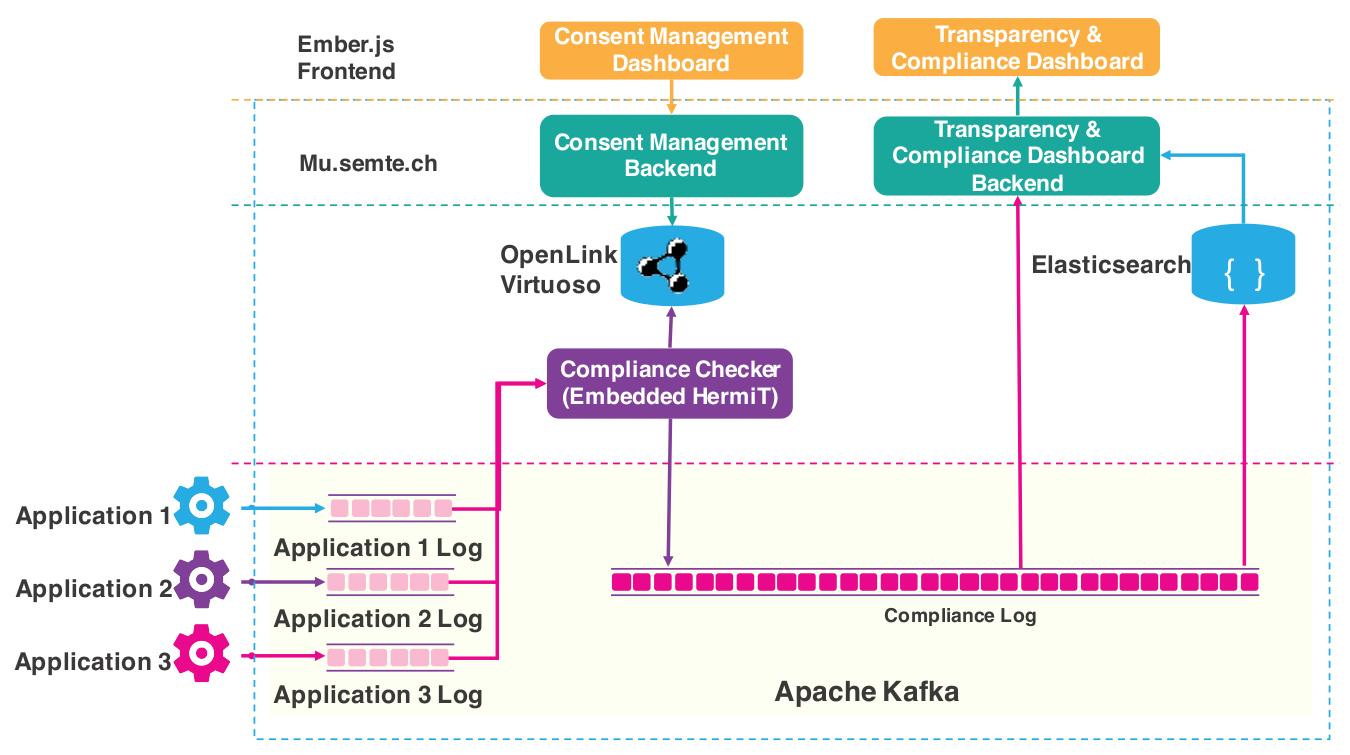
\includegraphics[width=\linewidth]{img/SPECIAL_architecture1.png}
    \caption{Overview of SPECIAL Architecture \cite{kirrane_scalable_2018}}
    \label{fig:SPECIAL-architecture1}
\end{figure}

The Usage Policy \cite{bonatti_special_2018-2} is used to represent data processing activities and is described in more detail in D2.5 \cite{bonatti_d2.5_2018}. The base policy uses OWL2 expressions to denote an intersection of personal data categories, processing operations, purposes, recipients, and storage. These can then be combined using OWL2 unions over multiple base policies with differing expressions. SPECIAL provides additional vocabularies for purposes, personal data categories, processing operations, and recipients for using with the Usage Policy based on its use-cases. The general form of a base policy is:
\begin{lstlisting}
ObjectIntersectionOf(
    ObjectSomeValuesFrom(spl:hasData SomeDataCategory)
    ObjectSomeValuesFrom(spl:hasProcessing SomeProcessing)
    ObjectSomeValuesFrom(spl:hasPurpose SomePurpose)
    ObjectSomeValuesFrom(spl:hasRecipient SomeRecipient)
    ObjectSomeValuesFrom(spl:hasStorage SomeStorage)
)
\end{lstlisting}
The storage expression is itself a policy comprising of OWL2 expressions specifying the storage location, duration, and interval. The general form of a storage policy is:
\begin{lstlisting}
ObjectIntersectionOf(
    ObjectSomeValuesFrom(spl:hasLocation SomeLocation)
    ObjectSomeValuesFrom(spl:hasDuration SomeDuration)
    DataSomeValuesFrom(spl:durationInDays Interval)
)
\end{lstlisting}

For a given policy $P_c$ representing activities permitted by given consent and policy $P_s$ representing processing activity, compliance is evaluated by checking whether $P_c$ complies with $P_s$ - which in OWL2 is checked by using a reasoner to check whether $P_c \subseteq P_s$. This is performed by using an algorithm \cite{bonatti_fast_2018,bonatti_richer_2019} in a semantic reasoner that is optimised for speed by only performing those operations associated with checking for compliance between policies.
An extension of the Usage Policy for representing additional requirements of the GDPR was discussed in the deliverable D2.6 \cite{bonatti_d2.6_2018}.

The activity is recorded in a log using the Policy Log vocabulary \cite{bonatti_special_2018-1}, represented in Figure. \ref{fig:SPECIAL-policy-log-vocabulary}, and is evaluated for compliance by using the reasoner in both ex-ante and ex-post phase. The Policy Log vocabulary, described in D2.7 \cite{kirrane_d2.7_2018}, reuses existing vocabularies such as DCAT and PROV \cite{lebo_prov-o:_2013}, and is used to record an immutable documentation of compliant activities and their legal basis in consent.

\begin{figure}[htbp]
    \centering
    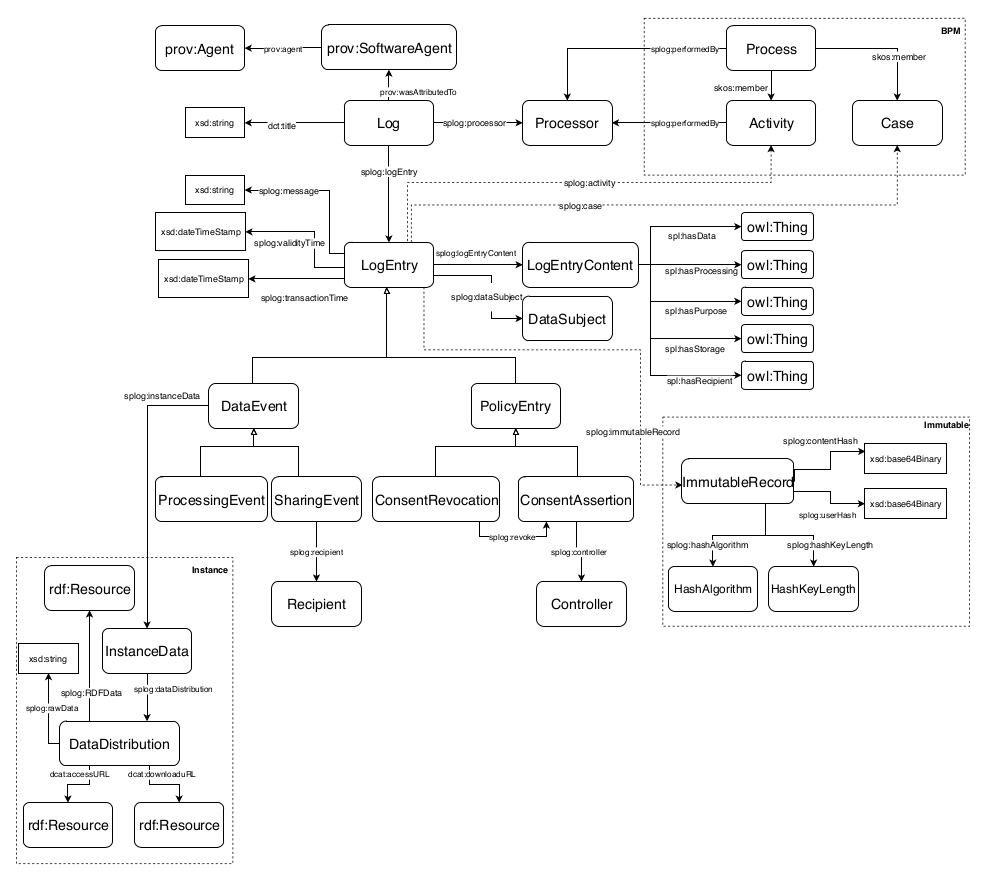
\includegraphics[width=\linewidth]{img/SPECIAL_logvocabulary.png}
    \caption{Overview of SPECIAL Policy Log Vocabulary \cite{bonatti_special_2018-1}}
    \label{fig:SPECIAL-policy-log-vocabulary}
\end{figure}

The methodologies associated with the vocabularies produced by the SPECIAL project are based on the utilisation of metadata in the compliance process \cite{wenning_compliance_2018}. The creation of policy vocabularies from use-cases is described through the public deliverable D1.5 \cite{bonatti_d1.5_2018}, with that of the log vocabulary provided in D3.2 \cite{kirrane_d2.7_2018}. The vocabularies created by the project are documented and publicly accessible online.

SPECIAL's work has also produced ODRL models for deontic representations of GDPR requirements through collaborations with other projects. The first of this is based on work with the Austrian SERAMIS\footnote{\url{https://cordis.europa.eu/project/rcn/189040/factsheet/en}} (Sensor-Enabled Real-World Awareness for Management Information Systems) project, which produced a web-based tool called PriWUcy for evaluating compliance assessments of GDPR articles \cite{agarwal_legislative_2018}.
The tool uses a model of the legislation created by parsing the legislation text and representing the obligations using ODRL. A set of preliminary assessment questions provides the inputs over which the model is applied to identify actions and obligations to be fulfilled as part of the assessment. The ODRL model, depicted in Figure. \ref{fig:SPECIAL-ODRL}, is extended to represent additional granularity of constraints of - Feature, Discretional, and Dispensation. The ODRL policies are associated with the text of the GDPR they represent through classes representing chapters, articles, and paragraphs within the text of the GDPR. The approach relies on identifying and representing assets, parties, actions, duties, and constraints using the developed ODRL model. More information on the tool can be found in the public deliverable D5.5 \cite{agarwal_d5.5_2017}.
\begin{figure}[htbp]
    \centering
    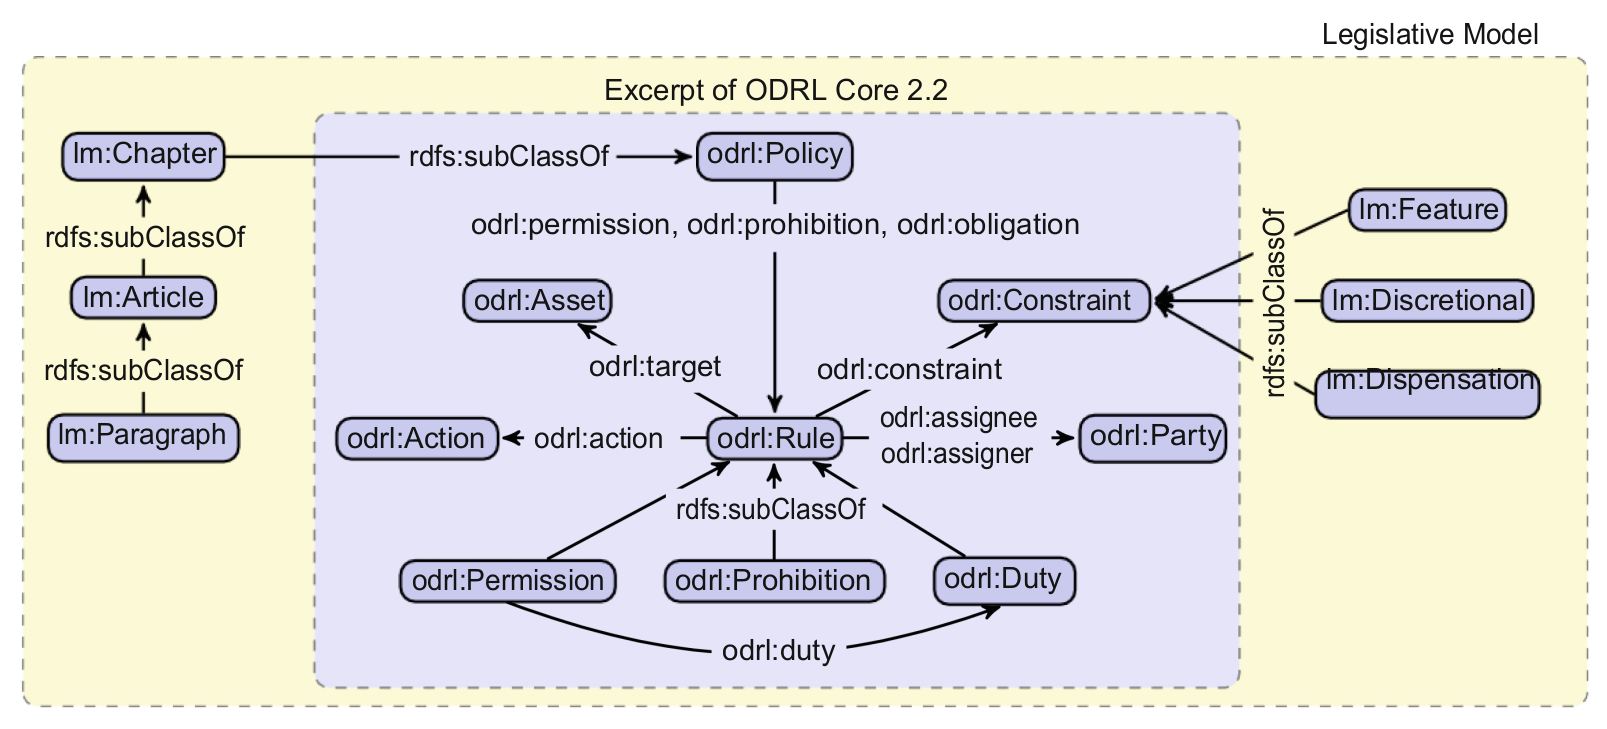
\includegraphics[width=\linewidth]{img/SPECIAL_ODRL.png}
    \caption{Extension of ODRL for representing GDPR obligations \cite{agarwal_legislative_2018}}
    \label{fig:SPECIAL-ODRL}
\end{figure}

The ODRL profile was further developed for modelling regulatory obligations and business policies based on GDPR towards compliance checking and providing explanations of the reasoning process \cite{vos_odrl_2019}. Additional classes and properties added include those relevant for specifying the legal bases, purpose, location, and safeguards associated with processing. Policies representing articles in the GDPR are checked against permissions by activities to perform a data processing operation. For example, the following listing shows a request for transfer personal data to a third country based on consent, which would be checked against the corresponding policy representing Article 46 of the GDPR. 
\begin{lstlisting}
<http://example.com/policy:bp-transfer> a orcp:Set ;
    odrl:profile <http://example.com/odrl:profile:regulatory-compliance> ;
    orcp:permission
    [ odrl:action orcp:Transfer ;
        orcp:data orcp:PersonalData ;
        orcp:responsibleParty orcp:Controller ;
        orcp:organisationType orcp:InternationalOrganisation ;
        orcp:sender <http://example.com/CompanyA_Ireland> ;
        orcp:recipient <http://example.com/CompanyA_US> ;
        orcp:recipientLocation orcp:ThirdCountry ;
        orcp:purpose orcp:PersonalRecommendations ;
        orcp:legalBasis orcp:Consent ;
        odrl:dataSubjectProvisions orcp:EnforceableDataSubjectRights ;
        odrl:dataSubjectProvisions orcp:LegalRemediesForDataSubjects
    ] .
\end{lstlisting}
Compliance is checked by converting the ODRL policies into InstAL, a domain-specific language for writing models based on events and states, which translates to Answer Set Programming (ASP) and is evaluated using a solver. When a policy is found to be non-compliant, explanations are generated based on `fluents' - facts that are true if present and false if absent - through a reasoning process. The implementation is publicly accessible through a hosted repository\footnote{\url{https://github.com/instsuite/instsuite.github.io/blob/master/gdpr.ial}}. An example of this is as follows:
\begin{lstlisting}
# fluents capturing justifications
type Article;
fluent permission(Subject,Article);
fluent prohibition(Subject,Article);
noninertial fluent supports(Subject,Article,Predicate,Object);
noninertial fluent lacks(Subject,Article,Predicate,Object);

# if enforceable data subject rights are defined, the term is true
article46_body_term2(Process) when
    triple(Process,dataSubjectProvisions,enforceableDataSubjectRights);
supports(Process,article46,dataSubjectProvisions,
        enforceableDataSubjectRights) when
    article46_body_term2(Process),
    triple(Process,dataSubjectProvisions,enforceableDataSubjectRights);

# otherwise the description lacks data, and non-inertial fluents are applied
lacks(Process,article46,dataSubjectProvisions,
        enforceableDataSubjectRights) when
    applies(Process,article46),
    not supports(Process,article46,dataSubjectPro
\end{lstlisting}

The second work is based on applying SPECIAL's GDPR compliance framework to the Austrian CitySPIN\footnote{\url{http://cityspin.net/}} (Cyber-Physical Social Systems for City-wide Infrastructures) project, which utilises linked data platforms to ingest data from multiple sources in a smart city scenario, and utilises it for data processing pipelines and analytics. An important component of the project is the management of consent which utilises SPECIAL's policies \cite{bonatti_special_2018-1,bonatti_special_2018-2} and compliance framework \cite{kirrane_scalable_2018}.
The auxiliary vocabularies provided by SPECIAL for purpose and data categories were extended for use-cases associated with CitySPIN \cite{fernandez_user_2019}, as depicted in Figure. \ref{fig:SPECIAL-CitySPIN}. 
The defined policies are checked in the ex-ante and ex-post phase using the SPECIAL compliance checking algorithm \cite{bonatti_fast_2018,bonatti_richer_2019}, with a prototype implementation demonstrating ex-ante compliance checking in ad-hoc widgets sharing personal data \cite{fernandez_privacy-aware_2019}. Details about the project and its implementation are available through its public deliverables D6.1 \cite{noauthor_d6.1_nodate} and D6.3 \cite{noauthor_d6.3_nodate}.

\begin{figure}[h]
    \centering
    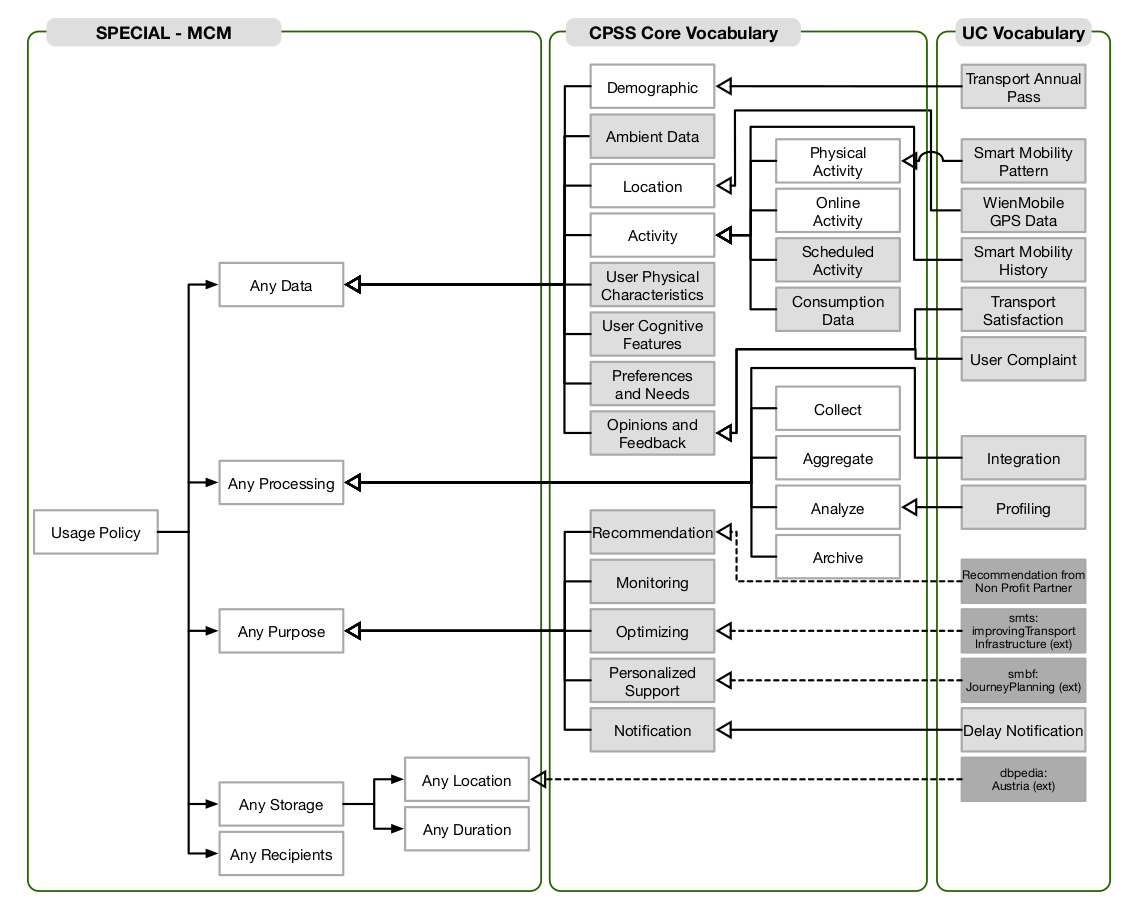
\includegraphics[width=\linewidth]{img/SPECIAL_CitySPIN.png}
    \caption{CitySPIN's extension of SPECIAL vocabularies \cite{fernandez_user_2019}}
    \label{fig:SPECIAL-CitySPIN}
\end{figure}

The use-cases utilised within the SPECIAL project and a discussion of their legal requirements can be found in the deliverables D1.5 \cite{bonatti_d1.5_2018} and D1.6 \cite{schlehahn_d1.6_2018}. A dashboard representing information of processing activities and consent was created to represent the logged information \cite{raschke_designing_2017}, whose usability and testing are described in deliverables D4.3 \cite{raschke_d4.3_nodate} and D4.4 \cite{milosevic_d4.4_2019}. Another visual interface for interactive consent was also developed based on presenting the components of a usage policy to the individual in an interactive format \cite{gritzalis_i_2019}. The interface provides visual representations of associations between purposes, processing, data categories, recipients, and storage which allows the individual to explore and choose their consent. It also offers visual paradigms such for representation of information as tabs, breadcrumbs, hierarchies, and graphs for visualisation and exploration of information. 

\subsection{MIREL}\label{sota:projects:MIREL}
MIREL\footnote{\url{www.mirelproject.eu/}} (Mining and Reasoning with Legal Texts) is an European H2020 Project that aims to create a framework for interpretation of legal texts into formal representations for querying norms, checking compliance, and decision support. The project uses semantic web to provide normative requirements \cite{gandon_normative_2017}, provide natural language processing over legal texts \cite{milagro_teruel_legal_2018}, and creating ontologies based on GDPR \cite{monica_legal_2018} for legal compliance \cite{palmirani_pronto:_2018-1} and reasoning \cite{palmirani_pronto:_2018}. The project also involves creation of icons for data protection based on the developed ontologies \cite{arianna_dapis:_2019}.
Information about the project is available through peer-reviewed publications and public deliverables\footnote{\url{http://www.mirelproject.eu/publications.php}}.
Details about the project and its developed resources, namely PrOnto, have  been described in publications, but are not open or publicly accessible at the time of writing this thesis.

The developed ontology is termed PrOnto (Privacy Ontology) \cite{monica_legal_2018}, and provides concepts within the GDPR associated with data types and documents, agents and roles, processing purposes, legal bases, processing operations, and deontic operations for modelling rights and duties. It reuses existing vocabularies \cite{palmirani_pronto:_2018} and has been applied within the Cloud4EU project\footnote{\url{http://www.agid.gov.it/cloudforeurope}} for legal compliance checking of eGovernment systems as well as the DAPRECO project (see \autoref{sota:projects:DAPRECO}).

PrOnto consists of modules representing (i) documents and data (depicted in \autoref{fig:PrOnto-data}), (ii) actors and roles, (iii) processing and workflow, (iv) legal rules and deontic formula, (v) purposes and legal bases. It also includes modules for risk analysis and measures, which it utilises to represent risk management processes such as DPIA as workflows \cite{palmirani_pronto:_2018}. Reasoning is utilised based on the deontic operators within the ontology, and violations are connected with the violated obligations thereby providing traceability towards the steps that created the violation. LegalRuleML is extended and used to represent the obligations and enable creation and rules for compliance.

\begin{figure}[htbp]
    \centering
    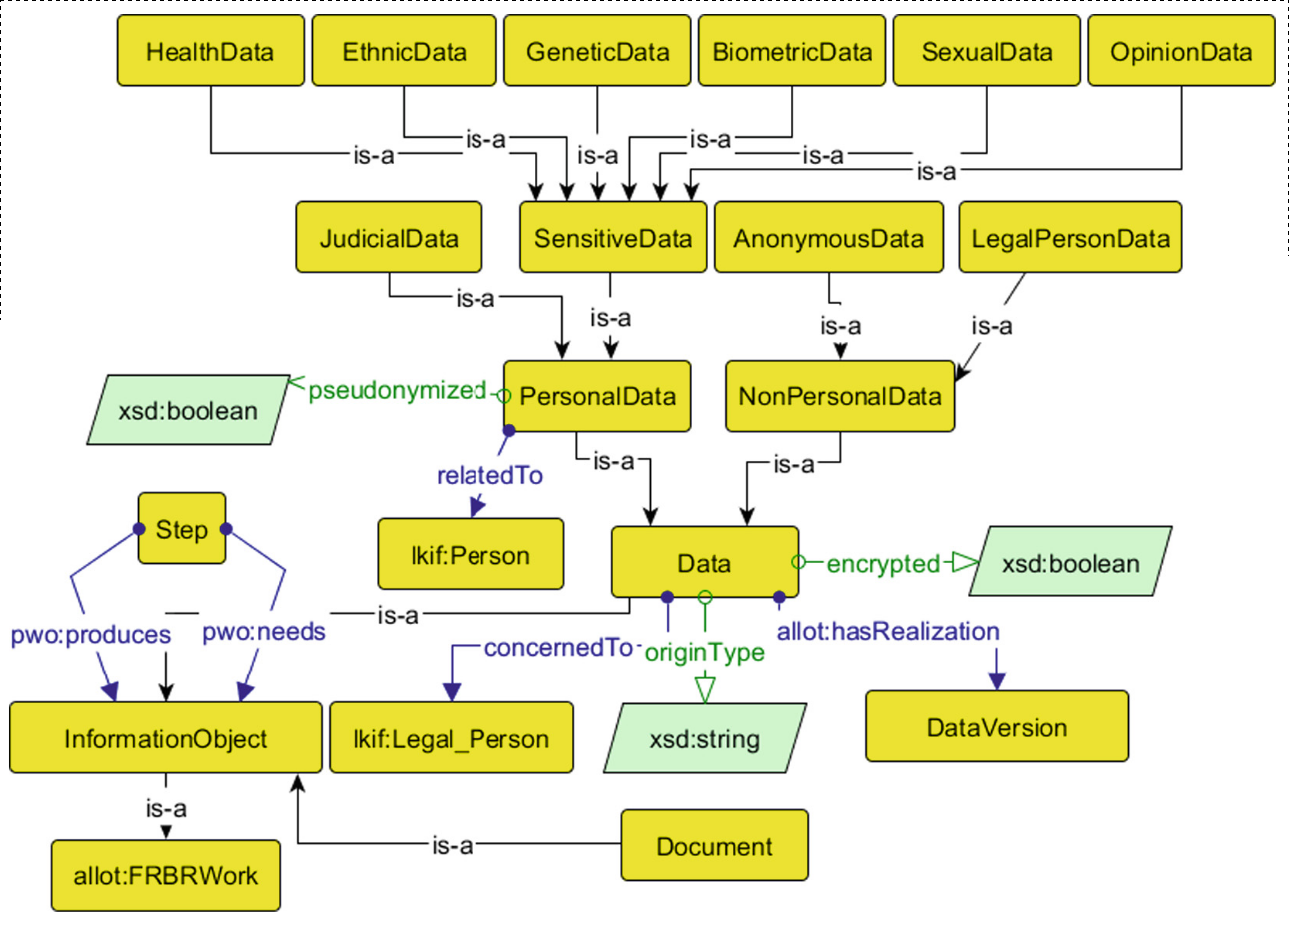
\includegraphics[width=\linewidth]{img/PrOnto_data.png}
    \caption{Data Categories represented in PrOnto \cite{palmirani_pronto:_2018}}
    \label{fig:PrOnto-data}
\end{figure}

PrOnto was developed using the MeLOn (Methodology for building Legal Ontologies) developed in the MIREL project \cite{palmirani_pronto:_2018,palmirani_pronto:_2018-1,monica_modelling_2018}. The methodology consists of the following ten recursive steps:
\begin{enumerate}
    \item Describe the goal of the ontology - in the case of PrOnto, these were: 
            (i) to model data protection legal norms starting from legal texts but including
also social norms, practitioner opinions or social behaviours;
            (ii) to build a legal ontology that is usable for legal reasoning;
            (iii) to build a legal ontology that is usable for web of data and information
retrieval.
    \item Evaluate ontology based on parameters/indicators derived from the goals. For PrOnto, these were - (i) coherence, (ii) completeness, (iii) efficiency, (iv) effectiveness, (v) usability, (vi) agreement.
    \item Reuse ontologies from SotA survey.
    \item List relevant terminology. For PrOnTo, the publication notes the creation of a glossry with relevant terminology and legal definitions extracted from legal sources.
    \item Use usable tools for legal experts. For PrOnto, these were tables and UML diagrams, and Graffoo to convert UML to OWL2.
    \item Refine and optimise the ontology by consulting with an expert. In PrOnto, these were manually performed by an ontology expert.
    \item Test the output. PrOnto was evaluated by legal experts in terms of completeness, effectiveness and usability.
    \item Evaluate the ontology. PrOnto used the OntoClean method to improve the ontology.
    \item Publish the document. PrOnto used the LODE tool to document the ontology.
    \item Collect feedback from community for agreement
\end{enumerate}

% TODO: references
An proof-of-concept application for detecting violations of the GDPR \cite{monica_modelling_2018} utilises PrOnto to model the legal concepts, along with Akoma Ntoso to model the legal text, LegalRuleML to model norms, and Regorous to apply LegalRuleML rules over BPMN and generate a report. The application utlises a web editor for modelling legal rules in connection with the legal text and ontology.
An example\footnote{The URI used in the namespace of the example, although using w3id, does not resolve, and therefore is not valid or is not publicly accessible.} of axioms extending LegalRuleML within PrOnto are depicted below:
\begin{lstlisting}
# Reparation
<owl:ObjectProperty rdf:about="https://w3id.org/ontology/pronto#repairs">
    <rdfs:domain rdf:resource="http://docs.oasis-
        open.org/legalruleml/ns/v1.0/metamodel#PenaltyStatement"/>
    <rdfs:range rdf:resource="http://docs.oasis-
    open.org/legalruleml/ns/v1.0/metamodel#PrescriptiveStatement"/>
</owl:ObjectProperty>

# Restriction: Obligation hasHeld CounterParty generated by a Right
<owl:ObjectProperty rdf:about="https://w3id.org/ontology/pronto#generates">
    <rdfs:domain rdf:resource="http://docs.oasis-
        open.org/legalruleml/ns/v1.0/metamodel#Right"/>
    <rdfs:range>
        <owl:intersectionOf rdf:parseType="Collection">
            <owl:Class rdf:about="http://docs.oasis-
                open.org/legalruleml/ns/v1.0/metamodel#Obligation"/>
            <owl:Restriction>
                <owl:onProperty rdf:resource="https://w3id.org/ontology/pronto#hasHeld"/>
                <owl:someValuesFrom rdf:resource="http://docs.oasis-
                    open.org/legalruleml/ns/v1.0/metamodel #AuxiliaryParty"/>
            </owl:Restriction>
        </owl:intersectionOf>
    </rdfs:range>
</owl:ObjectProperty>
\end{lstlisting}

\subsection{DAPRECO}\label{sota:projects:DAPRECO}
DAPRECO\footnote{\url{https://www.fnr.lu/projects/data-protection-regulation-compliance/}} (Data Protection Regulation Compliance) is an Luxembourgish project relating to the creation of a knowledge base for formal compliance with the terms and provisions of the GDPR. It aims to provide formalisms in deontic logic and natural language semantics for handling legal norms in written language. The project has researched correlation of standards with laws \cite{bartolini_towards_2016}, creation of an ontology to model concepts in the GDPR \cite{otake_using_2017}, modelling the norms of the GDPR using logic formalisms \cite{bartolini_legal_2018}, and annotating BPMN for GDPR compliance \cite{bartolini_enhancing_2019}.
The project involves collaborations with the MIREL project (see \autoref{sota:projects:MIREL}), particularly in the creation and utilisation of PrOnto for addressing GDPR \cite{monica_legal_2018,palmirani_pronto:_2018,palmirani_pronto:_2018-1,bartolini_enhancing_2019}. In turn, DAPRECO provides a practical application of PrOnto as an use-case for legal compliance over business activities \cite{bartolini_enhancing_2019,bartolini_agile_2019}.

While PrOnto represents a more mature and progressive deliverable of the project's ontology for GDPR, the earlier ontology - referred to as data protection ontology \cite{otake_using_2017} - is relevant for its modelling of the concepts and norms based on an draft of the GDPR. This ontology uses OWL2 to model the concepts of the GDPR and was specified to be a work in progress in its publication\footnote{It can be assumed the ontology is no longer being used or developed and was utilised in the development of PrOnto based on subsequent publications of the project \cite{bartolini_legal_2018,bartolini_enhancing_2019}.}.
Its methodology consists of using the structure provided by the Handbook on European Data Protection Law\footnote{2014 edition \url{https://publications.europa.eu/en/publication-detail/-/publication/eee277d3-d26f-4a18-825b-8e1fd80d2f0d/language-en}}, and consists of concepts associated with - data protection principles, rules of data processing constituting duties of data controller, and data subject's rights.
The ontology reuses concepts from LKIF Core \cite{hoekstra_lkif_2007} to represent rights, rules, legal and natural persons. It establishes relations such as \textit{hasObligation} between a \textit{Controller} and a \textit{LegalObligation} concept, and \textit{consentGrantedBy} between \textit{Consent} and \textit{DataSubject} - representing the relations derived from GDPR.
The ontology was evaluated using the the OOPS! tool \cite{poveda-villalon_oops!_2014}, and was documented using the LODE \cite{peroni_tools_2013}. The ontology can be accessed publicly\footnote{Link from \cite{otake_using_2017} \url{https://github.com/guerret/lu.uni.eclipse.bpmn2}} with documentation provided using LODE ontology documentation tool \cite{peroni_tools_2013}.
The Competency Questions (CQ) representing functional requirements for the ontology were used in its evaluation through SPARQL queries, and are follows:
\begin{enumerate}
    \item What are the obligations of a data controller?
    \item What are the functions of a data processor?
    \item What are the rights of the data subject?
    \item How do the rights of the data subject relate to the obligations of the data controller and the functions of the processor?
    \item How can a data subject interact and/or enforce their rights against a data controller?
    \item What are the possible fines and sanctions issued in response to violations by data controllers?
    \item Who supervises a data controller?
\end{enumerate}

Subsequent applications of PrOnto in the project utilises Reified Input/Output logic (RIO) \cite{robaldo_reified_2017} - a formalism for normative reasoning based on reification applied to natural language semantics. The rules are expressed using LegalRuleML and are associated with activities using BPMN. This is utilised to allocate tasks related to data protection to stakeholders, and to track compliance across different phases of a software development life-cycle.
The project uses these to create a knowledge base \cite{bartolini_agile_2019} with feedback from stakeholders by providing a human-readable version of RIO logic rules utilised to model the GDPR. 
The project also researchers automating the comparison of GDPR with the ISO by extracting RIO rules from their texts and analysing them for comparisons.
The resulting knowledge base is used in collaboration with the MIREL project to provide semantic extraction and annotation over ECHR (European Court of Human Rights) judgements \cite{cardellino_legal_2017}, as described in MIREL's deliverables D2.4 \cite{robaldo_livio_d2.4_2017}.

\subsection{BPR4GDPR}
BPR4GDPR\footnote{\url{http://www.bpr4gdpr.eu/}} (Business Process Re-engineering and functional toolkit for GDPR compliance) is an European H2020 project that aims to provide a a reference compliance framework for the GDPR. The framework is stated to provide specification of sophisticated security and privacy policies, modelling technologies and tools for the incorporation of provisions in process models and the resulting executable processes, and means for automating verification and alignment.
This is planned to be achieved using a set of mechanisms for automating the respective procedures and resulting in processes that are compliant by design.
The project intends to implement the concept of Compliance-as-a-Service (CaaS) by providing a set of tools that fit the needs of various organisations being subject to GDPR compliance.
Information about the project is available through peer-reviewed publications and project deliverables\footnote{\url{http://www.bpr4gdpr.eu/results/deliverables/}}.

The project uses an ontology to represent the information model utilised in its approach, as depicted in \autoref{fig:BPR4GDPR-model} \cite{lioudakis_d3.1_2019}. The ontology consists of concepts and relationships regarding:
\begin{itemize}
    \item DataTypes: all the types of data that can be used during the system's operation.
    \item Roles: roles that the system's users may hold.
    \item Operations: all the operations that may take place.
    \item OrganisationTypes: reflecting the different types of organisations, external or internal, actual or virtual, that may be involved in operations.
    \item OperationContainerTypes: representing functional components that offer a set of operations together.
    \item MachineTypes: types of machines that are used during the system's operation.
    \item EventTypes: types of events that may affect the operations and/or may require some action to take place in response.
    \item ContextTypes: specification of run-time constraints.
    \item Attributes: description of properties that characterise the entities.
\end{itemize}
The ontology is serialised using OWL2, and contains `default instances' representing a ready to use set of instances based on its use-cases, which are described in detail in deliverable D3.1 \cite{lioudakis_d3.1_2019}. 
\begin{figure}[htbp]
    \centering
    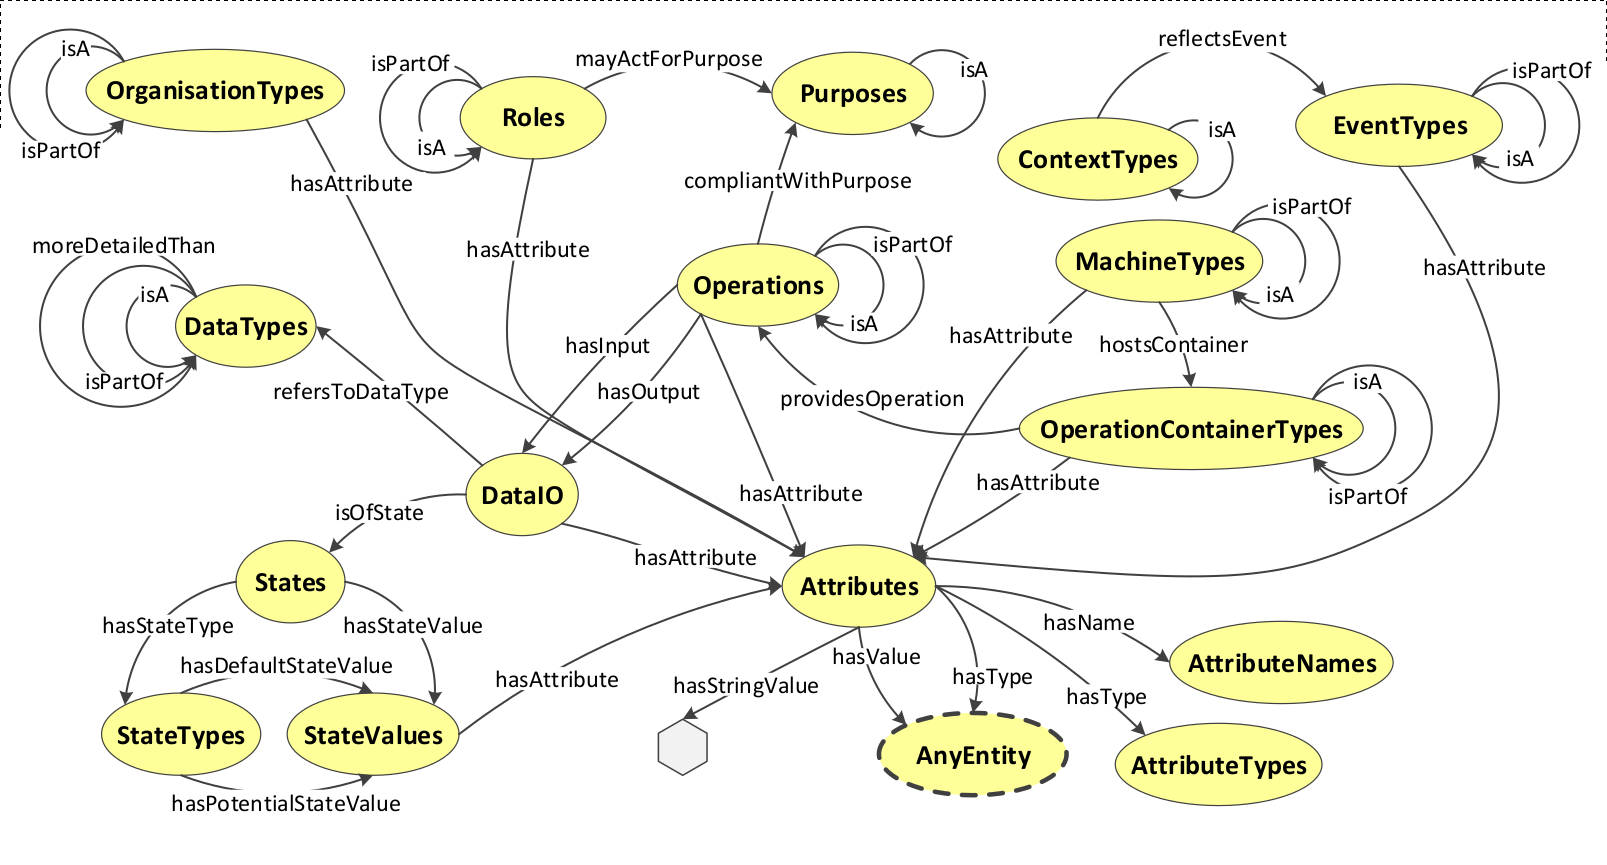
\includegraphics[width=\linewidth]{img/BPR4GDPR_model.png}
    \caption{Information Model Ontology in BPR4GDPR \cite{lioudakis_d3.1_2019}}
    \label{fig:BPR4GDPR-model}
\end{figure}

The compliance assessment is performed using the compliance meta-model ontology, as depicted in \autoref{fig:BPR4GDPR-compliance}, and described in detail in deliverable D2.3 \cite{dellas_d2.3_2019}. The compliance ontology is used to dictate and evaluate processes by considering them as worfkflows where actions or operations are connected to each other in terms of dependencies and data flows, are performed by an actor, and include assets or artefacts. Process mining is performed on the knowledge extracted from the event logs of information systems to discover, monitor and improve processes not assumed or modelled prior to the evaluation. This is then utilised to create a process monitoring architecture, which contains the following four sub-components of functionality:
\begin{itemize}
    \item The \textbf{pre-processing subcomponent} receives data from Data Management middleware as an input and updates and produces standard event logs for process mining. 
    \item The \textbf{conformance checking subcomponent} compares previously discovered models from those extracted from given event logs. The conformance depends on whether the process discovered from logs conforms to to the previously discovered or assumed process.
    \item The \textbf{rules subcomponent} retrieves policies from Security \& Privacy Policies module and converts them to a set of access control rules.
    \item The \textbf{model repair subcomponent} receives the to-be-repaired process models based on failed conformance checks, the converted rules, and the results of conformance checking as inputs, and identifies  parts of the process model not compliant with the rules. 
\end{itemize}

\begin{figure}[htbp]
    \centering
    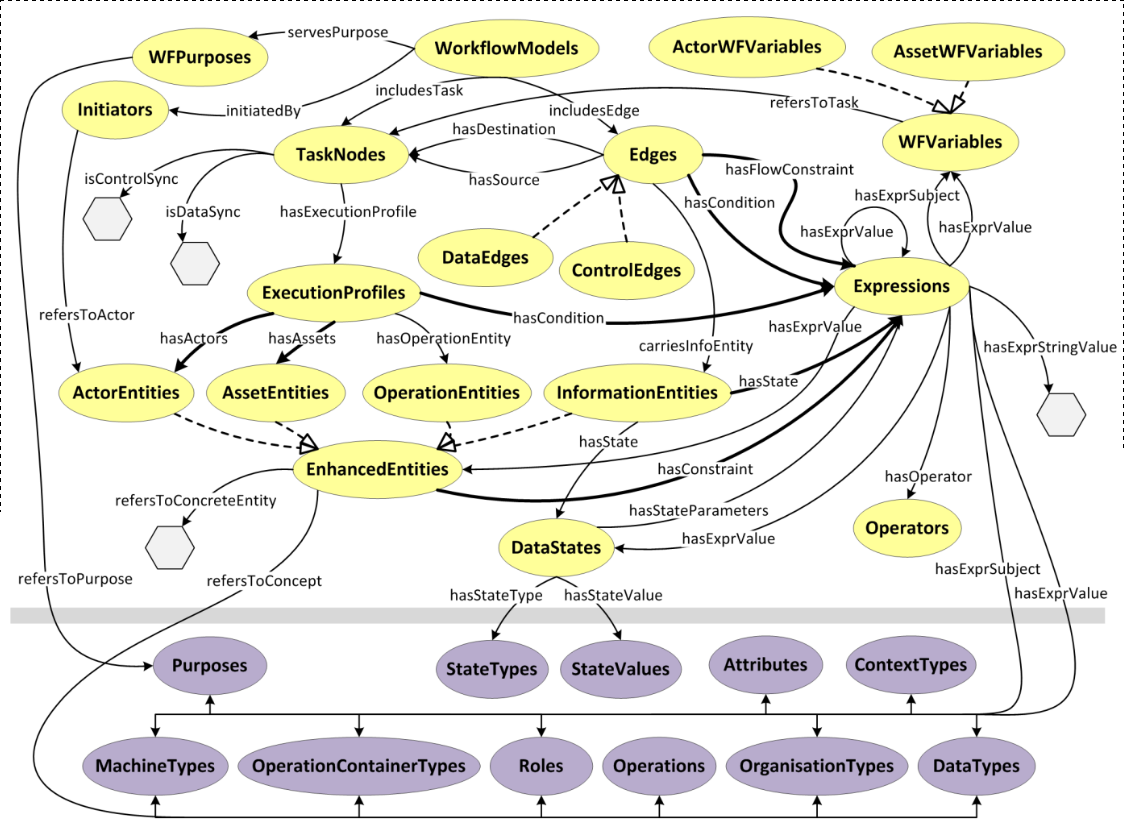
\includegraphics[width=\linewidth]{img/BPR4GDPR_compliance.png}
    \caption{Compliance meta-model ontology in BPR4GDPR \cite{dellas_d2.3_2019}}
    \label{fig:BPR4GDPR-compliance}
\end{figure}

The public deliverable D3.1 \cite{lioudakis_d3.1_2019} defines rules derived from the GDPR which represent the minimal set of configurations of the BPR4GDPR architecture before it is adapted to a particular use-case, i.e. its default configuration. The rules are as follows:
\begin{enumerate}[label={\textit{Rule\#\theenumi}}]
    \item  Nobody should have access to any data (secrecy by default)
    \item  An authorisation mechanism should be available and used in any access and use operation
    \item  A data breach must be reported within 72 hours starting when the controller has ascertained the
    breach
    \item  No data should be shared to third parties
    \item  If shared, data must be pseudonymised or anonymised
    \item  Stored data must be encrypted
    \item  Data subjects should have access to their data
    \item  No data processing should take place unless the data subject has provided consent
    \item  The means for updating consent must be provided, thus keeping consent information up to date
    \item  An easy way to revoke consent must be provided
    \item  If consent has been obtained, it should be tracked
    \item  Data subjects must be provided with adequate privacy notice
    \item  Data subject must be able to update or modify his/her own personal data
    \item  Personal data should be stored for no longer than required by the underlying law/regulation, as
    well as the duration of the purpose of the processing itself
    \item  The DPO should have broad access to personal data processing activities
    \item  The DPO should be involved in any data processing assessment
    \item  No actions may be taken without the prior consultation of the DPO
    \item  Access to personal information should be granular, according to the role and the functions of the
    person who is meant to access
    \item  Features to carry out data portability should be enabled
    \item  The system should allow to delete only personal data eventually considered as either not relevant
    for specific and imperative obligations of the controller or inaccurate
    \item  Any record of processing for each controller should be stored separately and accessed only by
    authorised users
    \item  The system should allow for the customisation of data retention periods according to the
    particularities of the collected data
    \item  Transfer of personal data must be tracked
    \item  System administrator’s logging activity should be tracked
\end{enumerate}

\subsection{Elluri et al.}
Elluri et al. \cite{elluri_knowledge_2018, elluri_integrated_2018} present an ontology of rules and obligations for cloud data providers and consumers based on the GDPR and for Payment Card Industry Data Security Standard (PCI DSS). The ontology for GDPR \cite{elluri_knowledge_2018} is comprised of concepts for components - `Consumers and Providers', `Fines and Enforcement', `Breach \& Notification', `Data Protection Officer', and `Data Subject'. This is combined with the ontology developed for PCI DSS and Clous Security Alliance (CSA) to provide a comprehensive combined ontology for addressing their combined legal requirements and obligations \cite{elluri_integrated_2018}. The resulting ontology, depicted in \autoref{fig:Elluri-ontology}, consists of concepts and relationships associated with stakeholders, obligations for providers and consumers, and security requirements. 
\begin{figure}[htbp]
    \centering
    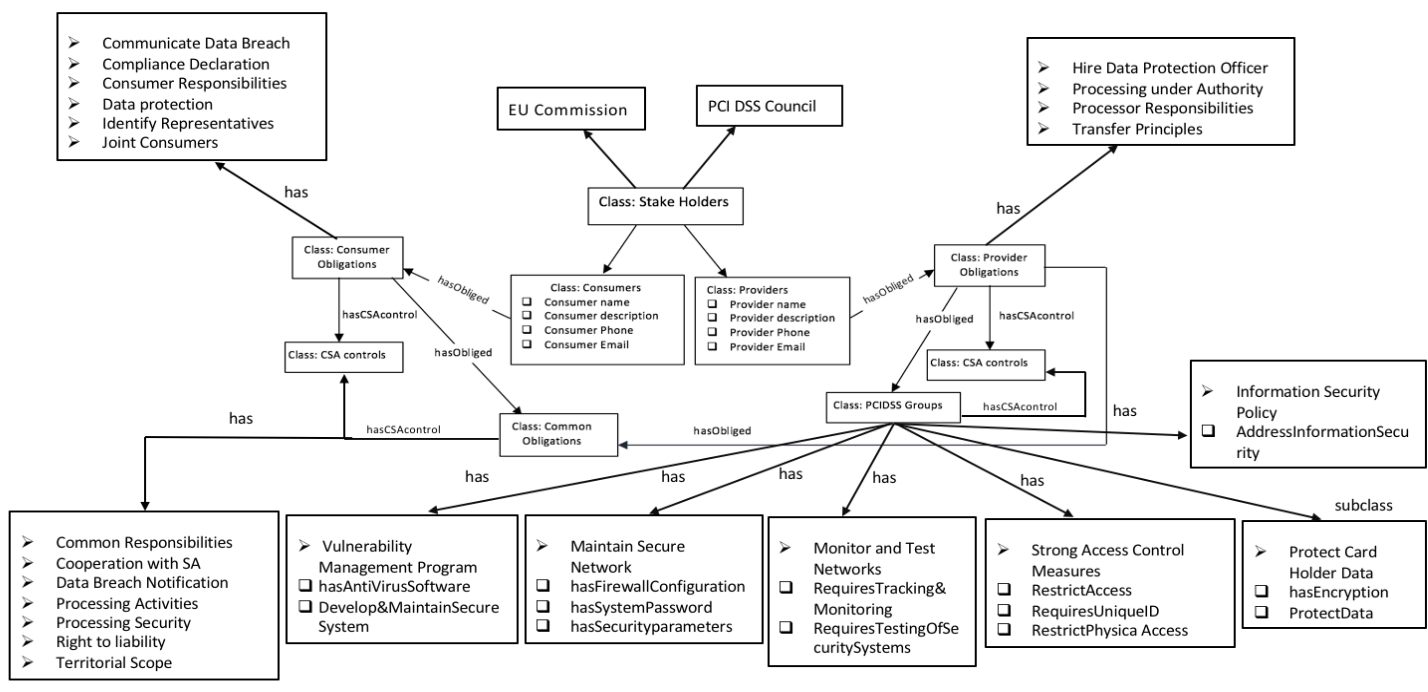
\includegraphics[width=\linewidth]{img/Elluri_ontology.png}
    \caption{Ontology of GDPR, PCI DSS, and CSA by Elluri et al. \cite{elluri_integrated_2018}}
    \label{fig:Elluri-ontology}
\end{figure}

The ontology development methodology included the following three steps: (i) Preprocessing, (ii) Ontology Development, and (iii) Validation. The preprocessing stage consisted of extracting relevant chapters and concepts from the text of the GDPR, PCI DSS, and CSA - and representing them using a preliminary ontology. These were then mapped with corresponding terms from the CSA ontology. This stage also involved identifying data protection rules in the form of permissions, obligations, dispensations, and prohibitions by using a keyword-based approach. Matching of concepts and rules was performed based using a tool that utilised text extraction and regular expressions to match contents with developed ontologies.

The validation of ontology utilised privacy policies of cloud service providers by comparing their text with the developed ontology using the developed tool. The extracted terms from policies were populated as instances of concepts in the developed ontology to provide an RDF representation of the policy. Apart from this description, the papers do not provide further details of the semantic representations or examples of the extracted information, nor an use-case demonstration of its capabilities. The ontology is referenced to be public and acessible\footnote{\url{https://ebiquity.umbc.edu/resource/html/id/377/Ontology-for-EU-s-General-Data-Protection-Regulation-GDPR}} \cite{elluri_knowledge_2018}, though it does not provide documentation or examples of its usage. Analysing the ontology shows instances of relevant chapters and articles within the GDPR applicable to PCI DSS and CSA, and declared as generic resources without reference to the actual text or IRI of the GDPR.

Related work within the same project by Joshi and Banerjee  \cite{joshi_automating_2019} concerns use of ontology to represent personal data categorisations and data privacy policies for automated enforcing of access control mechanisms regarding sharing of data with third parties through a blockchain. The data privacy policy, depicted in \autoref{fig:Ellur-PII-policy}, shows the concepts and relationships utilised to define information regarding processing. The privacy policy contains information about data collection purpose, data collected, protection measures, use limitations, consent requirements, and access control.
\begin{figure}[htbp]
    \centering
    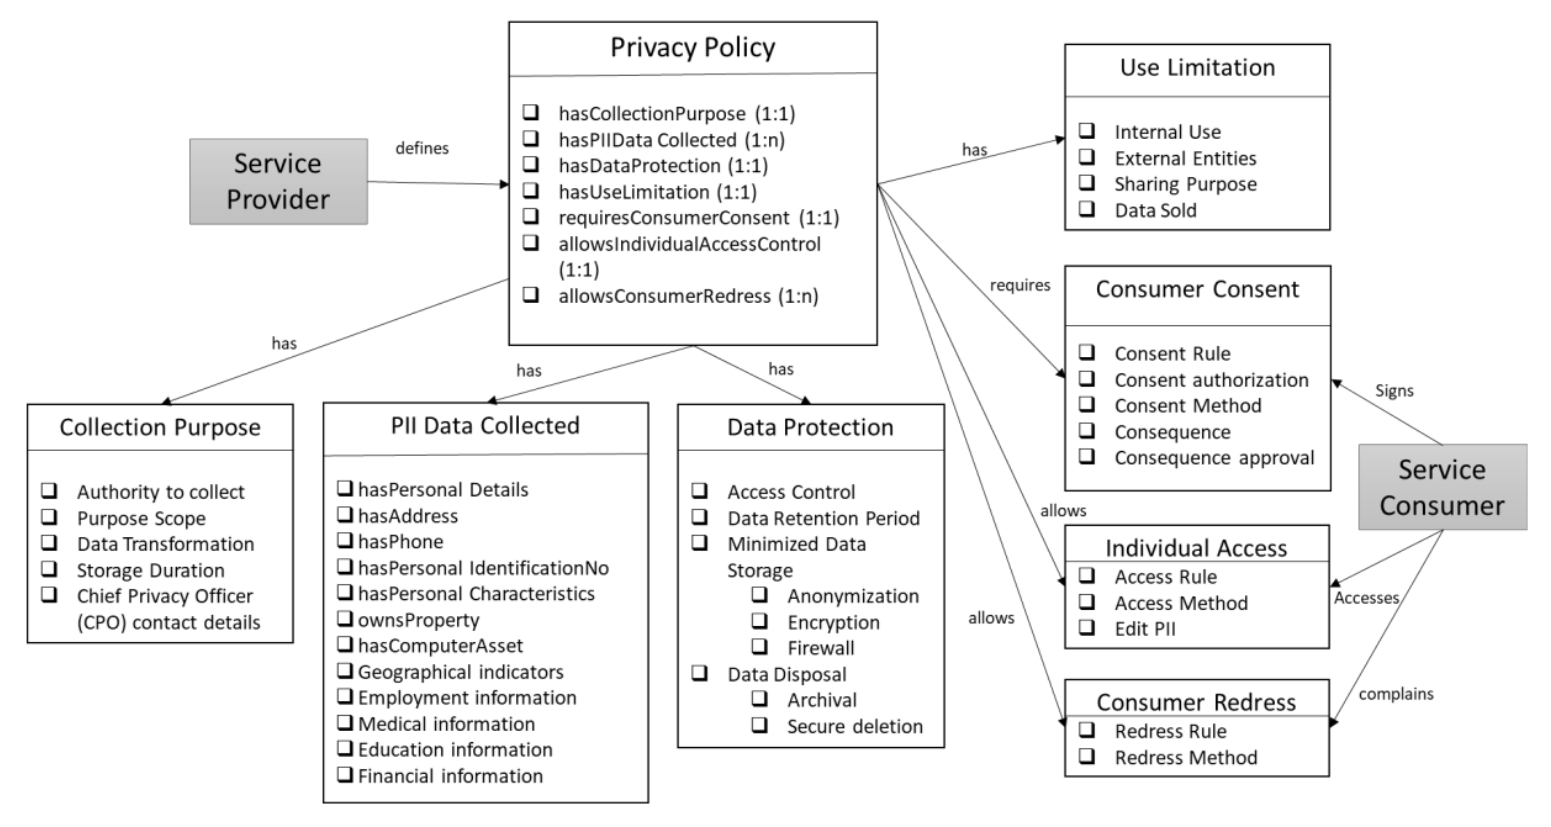
\includegraphics[width=\linewidth]{img/Elluri_PII_policy.png}
    \caption{Data Privacy Policy by Joshi and Banerjee \cite{joshi_automating_2019}}
    \label{fig:Ellur-PII-policy}
\end{figure}

The modelling of concepts includes some notably different relationships, such as the association of storage duration within collection purpose, usage limitation relating to data recipients, attributes associated with consent, and the inclusion of redress as a related concept. The developed ontology is utilised to extract and represent instances from privacy policies, enhance it using a reasoner, and to store the resulting access control representations in the blockchain. The work is based on the approach of utilising an existing privacy policy as a smart contract in the sharing of data between provider and consumer.
It is important to note that the work relates to the use of PII as opposed to personal data as defined by the GDPR. Furthermore, the policy does not encode information about rights as required by the GDPR.

\subsection{Ujcich et al.}
Ujcich et al \cite{belhajjame_provenance_2018} presented a data provenance model of the GDPR, depicted in \autoref{fig:Ujcich-ontology}, which utilises PROV-O \cite{lebo_prov-o:_2013} to represent activities and data in a semantic-web representation. The approach uses the activity `\textit{Justify}' to represent the rationale for processing personal data and has annotations depicting its starting and ending times, as well as a `\textit{Justification}' - which represents the legal basis of processing. The ontology focuses on the workflows involving exercising of rights under the GDPR, and provides examples of data rectification and withdrawal of consent utilising provenance.
\begin{figure}[htbp]
    \centering
    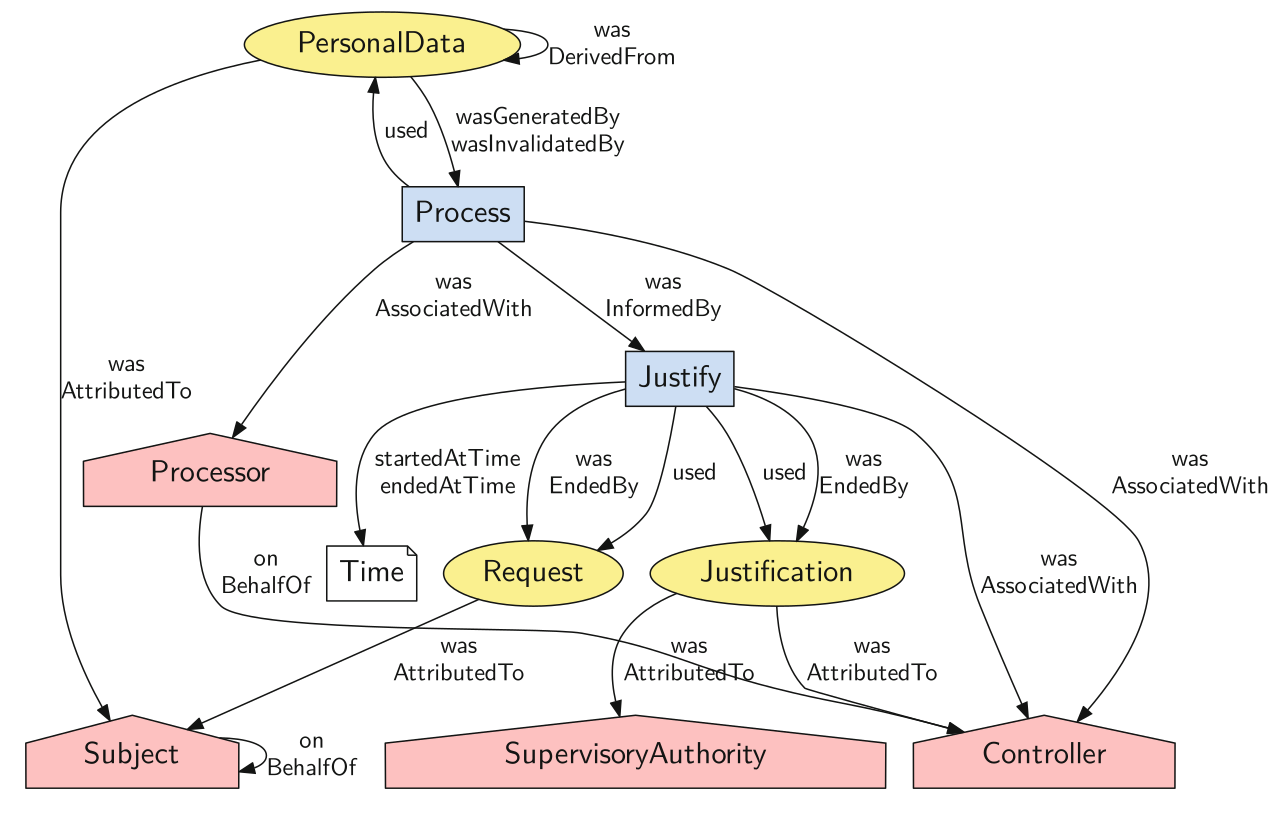
\includegraphics[width=\linewidth]{img/Ujcich_ontology.png}
    \caption{GDPR Data Provenance Model by Ujcich et al. \cite{belhajjame_provenance_2018}}
    \label{fig:Ujcich-ontology}
\end{figure}

The approach presented in the publication uses the notion of design patterns to describe the use of ontology in specific cases regarding the exercising of rights. The design pattern for provenance associated with consent does not associate the data directly with the consent owing to the reason of the data being potentially updated independent of consent. The design pattern is further extended to represent sharing data with a processor for marketing. The publication also provides a discussion on the verification of compliance based on provenance through questions which can be queried over the data represented using the presented ontology.

\subsection{Personal Information Controller Service (PICS)}
PICS is a project with the objective of enabling users to discover and control use of their personal data by utilising the platform as an authentication and management layer between service providers and personal information. The project architecture \cite{winckler_personal_2019} consists of three components: (i) personal data controller - provides an user interface allowing users to connect and mediate data to third-party services, (ii) ToS analyser - interprets terms of service and policies of providers using an ontology, and (iii) data mining traces of use - which enables discovery of web services utilising personal data shared with the service provider. The platform delegates the data storage to an external storage and does not store personal data itself. Authentication is performed at every interaction, and requires the user to provide physical authentication using a wearable device.

The ontology used by the ToS analyser \cite{benfenatki_towards_2019} consists of concepts associated with actions on data (such as deletion, disclosure, fusion, sharing), governance (laws, ownership, rights, terms of service), security strategies, and data protection. The ontology itself is not public or accessible and the publication does not provide complete details about its concepts or use beyond that of utilisation in the ToS analyser.

\section{Other Approaches for GDPR compliance}\label{sec:sota:gdpr-other}

\subsection{privacyTracker}
privacyTracker \cite{gjermundrod_privacytracker:_2016} is a framework that provides data traceability through privacy by design principles for GDPR compliance. The framework utilises policies to mediate access to information stored in the form of \textit{Customer Records}, and consists of 3 modules regarding data collection, data distribution, and data traceability. The \textit{Customer Record} is a XML document utilising XSD to store personal data, and contains two sections - a mandatory metadata section and an optional section. The metadata section contains fields for record identification, data tractability, and cryptographic controls. The optional section consists of fields indicating public data, private data which can be disclosed based on consent, and data provided by enterprise itself.

The record identification field contains a URI based on string concatenation of company name, user email address and auto-generated random identifier. This URI is unique throughout the framework, but changes when the data is distributed to another entity. In addition, the identification field also stores timestamps associated with record genesis, (local) record creation, and expiration. The data tractability fields record links to the entity that generated the record (backward-to-root reference), entities the record was obtained from (backward reference), and entities the record is disclosed to (forward reference). The cryptographic controls store a signed copy of the received record and a signature in the form of hash code of the complete record.
The distribution module enables sharing of data via an API through which granular requests can be made. Records of distributions are signed cryptographically and verified for tractability.
Enforcing rights is simplified by traversing the stored distribution records starting from the original record as root and moving towards the leaves.
A prototype of the implementation consisted of 6 companies and used MySQL and PHP as the technological framework. The records were stored using XML, which was then ingested into the database and queried using SQL.

The analysis of GDPR presented in connection with privacyTracker provide a list of requirements required to be satisfied by compliance frameworks, which are: Articles 5(1a), 5(1d), 6(1a), 6(1c), 7(1), 7(3), 12(1), 12(2), 14(1a), 14(1ac), 14a(2g), 15, 16(1), 17(1), 17(2a), 17a(1), 18(2), 19(2)). These provide the obligation to record and demonstrate evidence regarding handling and sharing of consumer data. 

\subsection{Metrics for Transparency by Spagnuelo et al.}
Spagnuelo et al. \cite{livraga_metrics_2016} define eight quality metrics for transparency regarding data processing associated with the GDPR.
In this context, transparency is defined based on quality factors of Informativeness, Understandability, and Accessibility associated with providing information, and Validity and Accessibility associated with providing mechanisms.
Each metric is associated with one or more questions that retrieve information regarding quality factors associated with its quantitative scoring.
The metrics provide a quantifiable representation of transparency in a system, and are used in a use-case to evaluate Microsoft Health-Vault - a commercial product.
The metrics are as follows - accuracy, currentness, conciseness, detailing, readability, availability, portability, and effectiveness.

\subsection{Metamodel for Privacy Level Agreements by Diamantopoulou et al.}
Diamantopoulou et al. present a metamodel for representing Privacy Level Agreements (PLA) with the aim of establishing contracts between controllers and individuals.
The metamodel, depicted in \autoref{fig:Diamantopoulou-metamodel}, represents privacy preferences using the concept of questionnaires, where each question refers to a specific data and the answer represents the individual's preferences regarding data sharing. The metamodel also associates preferences with threats, risks, and security measures through the data and controller. Requests for sharing data are associated with data and preferences, and can be accepted or denied based on the values of linked preferences.
The metamodel is specified to be designed for use-case in eGovernance scenarios where public administrators can provide data and value based on citizens preferences represented through the metamodel.
\begin{figure}[htbp]
    \centering
    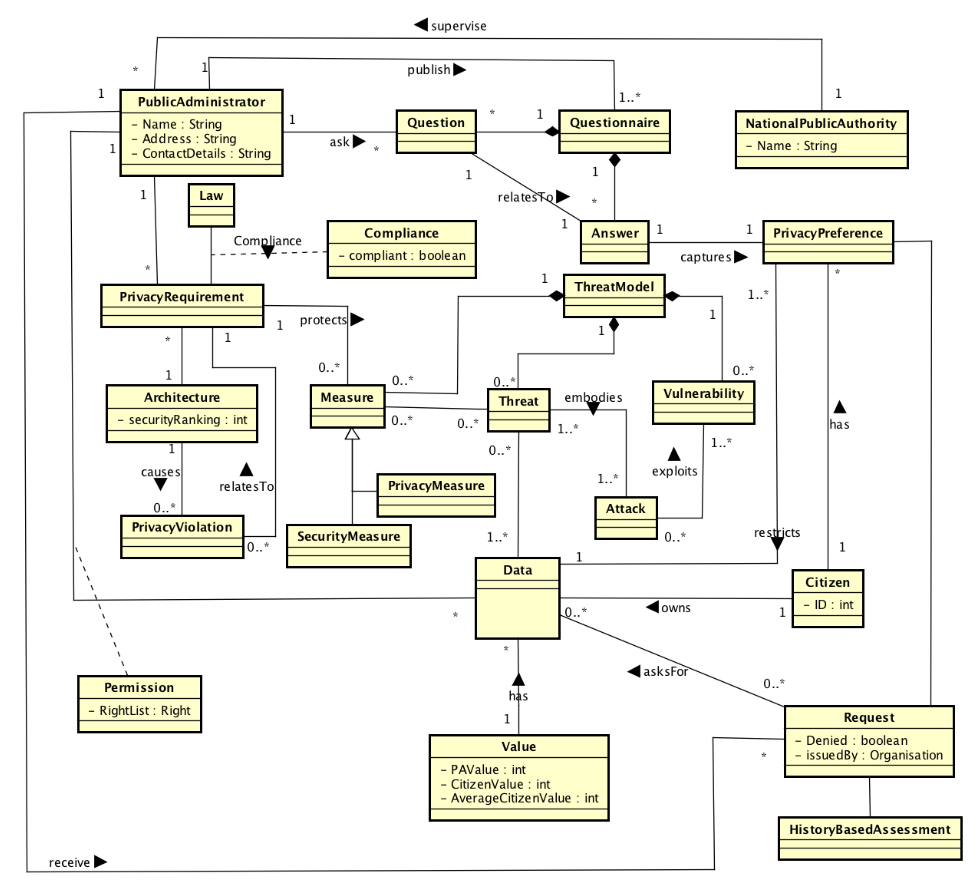
\includegraphics[width=\linewidth]{img/Diamantopoulou_metamodel.png}
    \caption{Metamodel for Privacy Level Agreements by Diamantopoulou et al. \cite{diamantopoulou_metamodel_2017}}
    \label{fig:Diamantopoulou-metamodel}
\end{figure}

\subsection{Robol et al.}
Robol et al. \cite{robol_toward_2017} proposed a modelling and reasoning framework based on socio-technical systems \cite{dalpiaz_security_2016} - an approach for incorporating interaction between people and technology. The proposed framework extends STS-ml - a goal-based modelling language provided in STS - with relevant concepts regarding privacy by design and GDPR compliance. The extended modelling language consists of three views - social, information, and authorisation - based on concepts and context of interactions between them. Social views incorporate actors and their goals and documents, as well as delegations and transmissions. Information views consist of associating actors with information and the tangible documents. Authorisation views consist of interactions with actors based on authorisations which are validated by legal basis over some information towards a particular goal. The modelling concepts are explained in the publication using a health-domain use-case.

Reasoning is based on using the concepts in policies that are then validated for compliance. The policies are based on formal representations of rules based on conditions and constraints for compliance, and the notion of \textit{well-formedness} of models. One notable aspect of this work is the use of concepts from socio-technical approaches to represent GDPR concepts. In particular, goal is used to simulate purpose, actors are used to conceptualise individuals and controllers, and authorisation is used to simulate valid legal basis. The approach enables use of STS modelling and reasoning to develop rules for expressing GDPR compliance requirements and validations.

\subsection{Ayala-Rivera and Pasquale}
Ayala-Rivera and Pasquale \cite{ayala-rivera_grace_2018} proposed a 6 step approach that links GDPR obligations with privacy controls for compliance and focuses on utilisation of data protection principles in activities. The approach, called GuideMe and depicted in \autoref{fig:Ayala-GuideMe}, is based on eliciting requirements from a business perspective and moving towards encapsulating them into compliant solutions. The first step consists of conducting a data audit to recognise all sources and instance of personal data, its storage, legal basis, and sharing, and identification of use in activities and their risks. The second step is a gap analysis to identify systems and processes that need remedial actions based on their violations of GDPR obligations. The third step utilises the results of gap analysis to establish plans for incorporating privacy controls towards obtaining compliance with the GDPR. The fourth step reviews the implementation plan with stakeholders, while the fifth step implements the corrective actions. The sixth and final step is the evaluation of implemented actions with experts.
\begin{figure}[htbp]
    \centering
    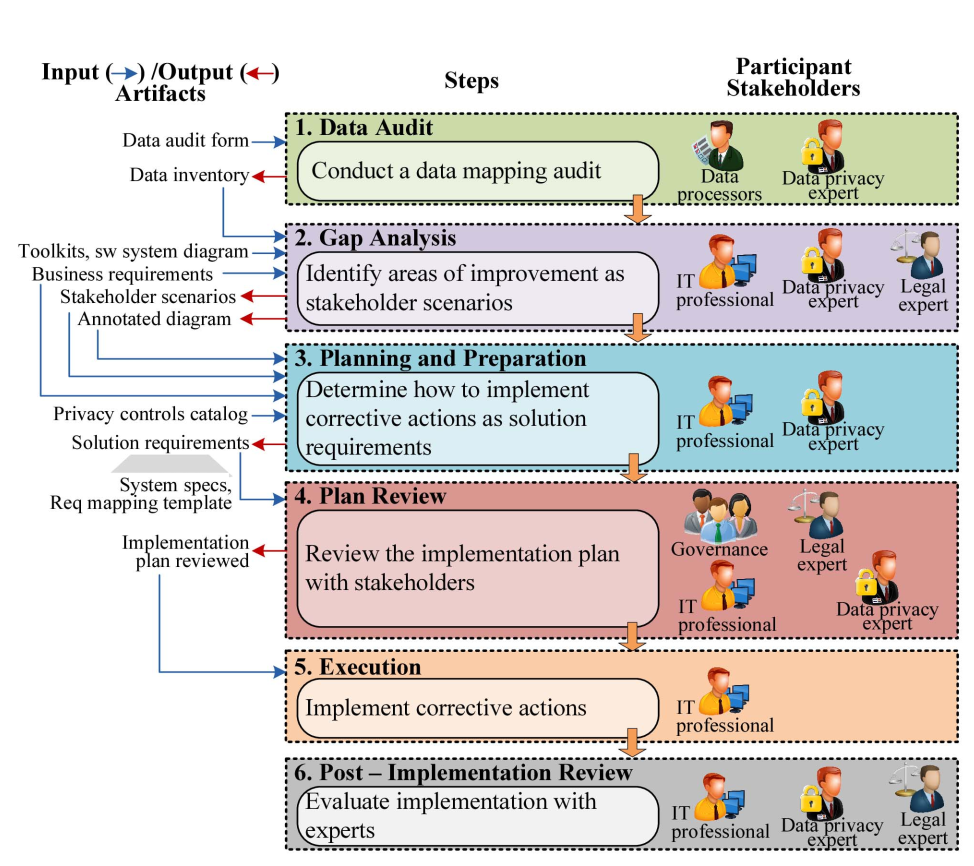
\includegraphics[width=\linewidth]{img/Ayala_GuideMe.png}
    \caption{GuideMe approach by Ayala-Rivera and Pasquale \cite{ayala-rivera_grace_2018}}
    \label{fig:Ayala-GuideMe}
\end{figure}

The publication provides examples through use-cases, stakeholder scenarios, and presents the application of data protection principles in each of GuideMe's steps. It also provides an examples utlising a template containing placeholders for incorporating legal obligations into business requirements. Evaluation of the implemented measures is explained through the example of scenarios which used SMART questionnaires to analyse and validate the corrective actions.

\subsection{Basin et al.}
Basin et al. \cite{basin_purpose_2018} proposed an approach that aligns purpose as defined by the GDPR with a business process, and uses formal models of inter-process communication to audit GDPR compliance. The approach also uses models of data flows to derive privacy policies. 
The definition of business process used in the approach ...

% non sem-web
\subsection{RestAssured}
RestAssured\footnote{\url{https://restassuredh2020.eu/}} is an European H2020 project that aims to enable secure data processing in the cloud with sticky policies for decentralised data lifecycle management.
The project aims to achieve this by using run-time models for data protection assurance and automated risk management. Run-time detection, prediction, and prevention of data protection violations is achieved by using a catalogue of risk patterns representing data protection vulnerabilities of cloud systems \cite{palm_modelling_2018,braubach_using_2018}. The pattern meta-model and its validation is described in detail in the deliverable D5.1 \cite{noauthor_d5.1.pdf_nodate}. Information about the project is available through peer-reviewed publications and publicly available deliverables\footnote{\url{https://restassuredh2020.eu/publications/}}.
\begin{figure}[htbp]
    \centering
    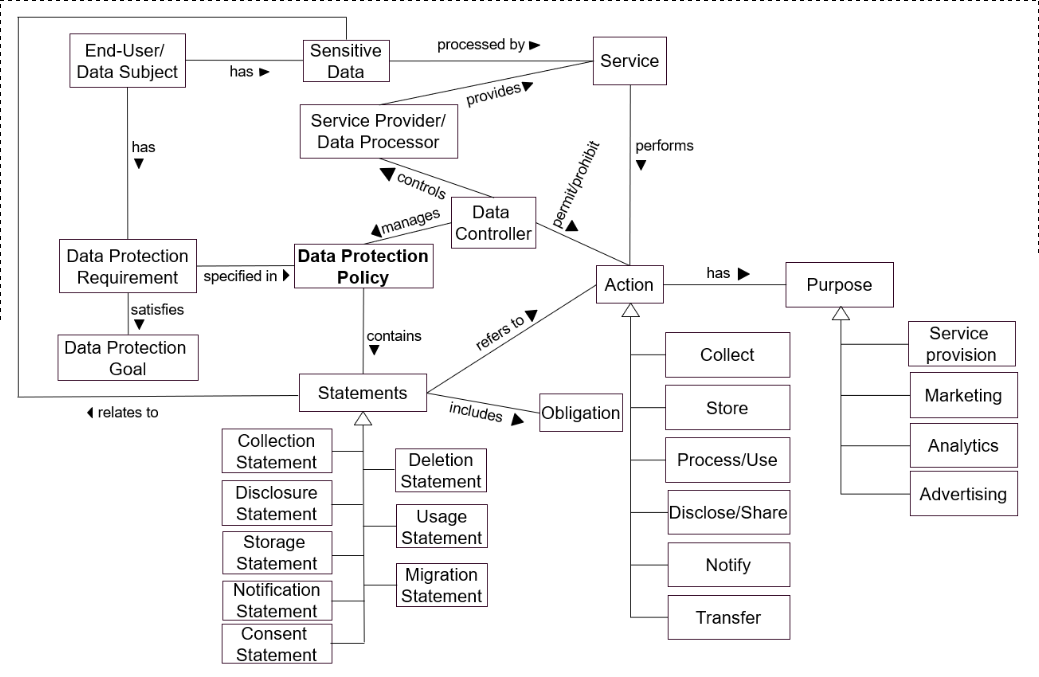
\includegraphics[width=\linewidth]{img/RestAssured_model.png}
    \caption{Model of policy specification framework in RestAssured \cite{noauthor_d6.1.pdf_nodate}}
    \label{fig:RestAssured-model}
\end{figure}

% non sem-web
The project addresses GDPR specifically through a conceptual model incorporating concepts necessary for compliance, as depicted in \autoref{fig:RestAssured-model} \cite{noauthor_d6.1.pdf_nodate}. The model is utilised in a data protection policy specification consisting of a data protection contract, sticky policies, and specification of obligations. The model is utilised to provide a customised privacy policy that allows users choice of preferences for selected services \cite{gritzalis_privacy_2019}. The data protection contract is composed of 4 main parts:
\begin{enumerate}
    \item A description of the Service that needs to access the data
    \item A specification of the data that is needed to be accessed by the service and whether this access is mandatory
    \item A list of usages, where a usage is composed of a textual description that describes the purpose of this usage(example: statistics, marketing) and the associated action (example: store, read, etc.) as well as a list of needed data types
    \item A specification of data that will be published by the service
\end{enumerate}
The obligations are defined based on their enforcement in relation to access control (before, at same time, after), and are specified with three pieces of information: (i) obligation type (before, after, with), (ii) event trigger, and (iii) action to be performed. The serialisation of obligations is done using XACML 3.0.
The deliverable D7.1 \cite{noauthor_d7.1.pdf_nodate} refers to the use of RDF to represent the concepts and relationships as a graph, which consists of three layers:
\begin{enumerate}
    \item \textbf{A core model}: the schema that captures the fundamental concepts, e.g. assets, roles, threats, and their relationships.
    \item \textbf{Domain models}: datasets that encode domain- specific knowledge, e.g. detailed threats and their possible control strategies.
    \item \textbf{System models}: that represent an actual system upon which the risk assessment is being performed.
\end{enumerate}

% non sem-web
\subsection{DEFeND}
DEFeND\footnote{\url{https://www.defendproject.eu/}} (Data Privacy Governance for Supporting GDPR) is an European H2020 project that aims to create a platform for providing services to organisations in the context of GDPR compliance. The platform is stated to provide services regarding data management and governance, data breach reporting, process management, along with GDPR planning and reporting. The peer reviewed publication \cite{piras_defend_2019} presents more details about the architecture of the project and its various components.

The Data Assessment Component (DAC) consists of the Organisation Data Collection (ODC) module which uses an questionnaire to collect information about organisational scope, data processing, processes, and activities - and is used to evaluate the organisation with relevant aspects of the GPDR. The questionnaire responses from ODC are given to the Assessment Translator (ATr) module which converts them to an XML-schema in order to create Data Assessment Model (DAM) - which is a goal-based requirement engineering model of actors, assets, establishments and data flows.

The DAM is used by the Data Privacy Analysis Component (DPAC) to perform analysis about DPIA, Data Minimisation, Privacy-by-Design/Default, and Threat mitigation. The outcome of the analysis is a Data Privacy Model (DPC), which is utilised to specify and evaluate both at design and run-time the operations of consent management, data access rights, security and privacy technologies. The project also aims to create a dashboard to provide organisations with control and monitoring of operations to achieve GDPR compliance, and to enable data subjects to interact with the platform based on consent.

% non sem-web
\subsection{OPERANDO}
OPERANDO\footnote{\url{www.operando.eu/}} (Online Privacy Enforcement, Rights Assurance \& Optimisation) is an European H2020 project that aims to provide a platform for users to specify preferences via a dashboard, which is then compared with online service providers privacy policies and converted into access control rules.
The deliverable D3.1 \cite{noauthor_d3.1-guidelinesonlegalaspectsv2.0_77_289.pdf_nodate} describes the legal requirements of the GDPR in the context of OPERANDO's objectives, while deliverable D6.4 \cite{noauthor_d6.4finalproductversionofprivacyenhancedtoolsv1.0_77_366.pdf_nodate} describes the architecture and working of privacy tools.
Information about the project is available through peer-reviewed publications and public deliverables\footnote{\url{http://www.operando.eu/servizi/moduli/moduli_fase01b.aspx}}.

The platform operates in an online environment and uses APIs between services which pass information using JSON. An User Privacy Policy (UPP) \cite{noauthor_d6.7finalproductversionofsecurityawaretoolsv1.0_77_378.pdf_nodate} is stored in the platform database and represents the user's preferences (and consent). The UPP records preferences using fields for information identifiers, personal data category, ranked preference (0 to 10, higher indicating greater concern), role (of person acting on data), action (performed on data), purpose, and recipient. The UPP also contains information on access policies created based on comparing the user's preferences against an online service provider's privacy policy. 

The online service provider's privacy policy (OSP) \cite{noauthor_d6.7finalproductversionofsecurityawaretoolsv1.0_77_378.pdf_nodate} consists of fields defining workflows and contained steps with information about requester subject (role of service provider), requested data, and action to be performed. The OSP also contains information about access policies for which the service provider has privileges to perform the requested operations in specified roles. Information about how the UPP and OSP are utilised in an API to enact an access request is provided through the deliverable D6.4 \cite{noauthor_d6.4finalproductversionofprivacyenhancedtoolsv1.0_77_366.pdf_nodate}.

% non sem-web
\subsection{PDP4E}
PDP43\footnote{\url{https://www.pdp4e-project.eu/}} (Methods and Tools for GDPR Compliance through Privacy and Data Protection Engineering) is an European H2020 project that aims to provide tools and guidance for incorporating privacy and data protection into software development life-cycles (SDLC) to implement data protection by design. Currently, the project lists one deliverable on its website, D2.1 \cite{noauthor_pdp4e-d2.1_multistakeholder_nodate}, which provides information on the legal analysis of GDPR in terms of requirements and obligations for software, and identifies the various roles and responsibilities within the context of SDLC. 


% non sem-web, relevant
\subsection{PoSEID-on}
POSEID-on\footnote{\url{https://www.poseidon-h2020.eu/}} (Protection and control of Secured Information by means of a privacy Enhanced Dashboard) is an European H2020 project that aims to safeguard the rights of data subjects
while simultaneously supporting organisations in data management and processing while ensuring GDPR compliance.
Its objective is to create a Privacy Enhancing Dashboard for personal data protection using an implementation of permissioned blockchain and smart contracts to provide accountability, transparency and compliance.
The project aims to develop technologies for automated detection of unexpected and potentially harmful behaviours in order to monitor privacy risks and notify threats to data subjects during transactions.
Information about the project is available through its public deliverables\footnote{\url{https://www.poseidon-h2020.eu/documents/}}.

Deliverable D2.1 \cite{noauthor_poseid-on_d2.1-use-cases-analysis-and-user-scenarios-v1.00.pdf_nodate} provides information on use-cases considered within the project with their user stories, personal data required in the use-case, and third parties involved. Deliverable D3.1 \cite{noauthor_d3.1_final-version_poseidon_v10.pdf_nodate} presents the architecture of the PoSEID-on, with information about the smart contract utilised on the permissioned blockchain. The smart contract supports permissions regarding requesting, granting, revoking, notifying, checking, and accessing permissions regarding use of PII. Each permission event is logged to the blockchain and consists of the data processor, data subject, and personal data field involved. Deliverable D4.3 \cite{noauthor_d4.3-rmm-and-pda-v1.0-final.pdf_nodate} describes use of natural language programming approaches to detect PII in stored data as a measure of risk detection and management.

% non sem-web, relevant
\subsection{STAR \& STAR II}
STAR\footnote{\url{https://projectstareu.wordpress.com/}} (Support Training Activities on the data protection Reform) is an European project that had the aim to provide materials to support training of DPAs and DPOs for the GDPR. To this end, it has created and published its resources consisting of training materials in an open and publicly accessible form\footnote{\url{http://www.project-star.eu/training-materials}}. The resources also provide a compliance checklist \cite{noauthor_gdpr_2019-1}, which provides a list of questions and criterion to assess preparedness with the requirements of the GDPR. 

\section{Approaches of Relevance}\label{sec:sota:other}
% non sem-web
\subsection{My Health My Data (MHMD)}
My Health My Data\footnote{\url{http://www.myhealthmydata.eu/}} (MHMD) is an European H2020 project that aims to develop infrastructure based on blockchain and smart contracts, which provide personal data accounts in the cloud that can be managed using dynamic consent interfaces and provide peer-to-peer connections between stakeholders. The project uses blockchain to log data transactions in a secure, transparent, and accountable manner, while using de-identification and encryption to protect identity and sensitive information. The safety and security of the data is tested using re-identification and penetration simulations.
Information about the project is available through peer-reviewed publications and public deliverables\footnote{\url{http://www.myhealthmydata.eu/publicdeliverables/}}.

The project is applied over the use-case of health data and devices, described in deliverable D1.1 \cite{noauthor_d1.1_initial-list--main-requirements.pdf_nodate}, and uses an ontological resource to model the common data ontology - described more in its deliverable D4.2 \cite{teodoro_d4.2-mhmd-ontological-resources.pdf_2018}. The common data ontology consists of modular health data ontologies representing synthetic data shared by the project's commercial partners as an use-case.
Access to the data is provided through an API that includes parameters describing the requested data category as well as consent descriptions. The API returns matching datasets which can then be utilised for data processing activities. The consent description parameter of the API is a text field consisting of values such as ``synthetic data'' and ``fully anonymised'' which reflect the state of data and its requirements in terms of consent. 

Though the project aims to utilise the GDPR as a source of legal requirements and strives to design its framework to meet compliance requirements by both design and default, there is no publicly available information regarding the specifics of how GDPR compliance is achieved or represented.
It focuses on the privacy preserving and security aspects of data storage by using technological solutions such as access control and transparent logging to design specifications based on legal requirements.
The project does explores the impact of GDPR of storing data in a blockchain, especially regarding the right to be forgotten \cite{bayle_when_2018}.

% non sem-web, relevant
\subsection{PAPAYA}
PAPAYA\footnote{\url{https://www.papaya-project.eu/}} (PlAtform for PrivAcY preserving data Analytics) is an European H2020 project that aims to provide privacy preserving techniques and technologies for performing analytics tasks on encrypted data by untrusted third-party data processors. The project uses the obligations of the GDPR to structure its outcomes in terms of Privacy Enhancing Technologies (PETs) which are provided through an intoperable platform. The project focuses on the application of privacy by design principle to provide usability, transparency, and auditability to end users regarding the processing of their data. Information about the project is available through peer-reviewed publications\footnote{The deliverables listed at \url{https://www.papaya-project.eu/deliverables} are not publicly accessible at the time of writing this thesis.}.

% non sem-web, relevant
\subsection{SMOOTH}
SMOOTH\footnote{\url{https://smoothplatform.eu/}} is an European H2020 project that aims to assist micro enterprises become compliant with the GDPR by designing and implementing tools for awareness about GDPR obligations and analysing their level of compliance with the new data protection regulation.
The objectives of the project include creation of a platform for automatic assessment of privacy protection documents (including privacy policies), stored data, and the processing of personal data on the website or mobile apps to create a compliance report. Further details about the project are currently not available.

% non sem-web
\subsection{SODA}
SODA\footnote{\url{https://www.soda-project.eu/}} (Scalable Oblivious Data Analytics) is an European H2020 project that aims to provide tools for performing analytics over encrypted data at large scales while providing compliance with the GDPR. The project will utilise use-cases within the health domain to demonstrate the privacy-preserving aspects of its technologies. SODA incorporates requirements of the GDPR and provides guarantees regarding compliance through the use of its tools and technologies. The analysis of legal requirements arising from the GDPR and the role of SODA in addressing them is presented in deliverable D3.1 \cite{spindler_d3.1_2017}. Further information about the project is available through peer-reviewed publications and public deliverables\footnote{\url{https://www.soda-project.eu/deliverables/}}.

% non sem-web, relevant
\subsection{DECODE}
DECODE\footnote{\url{https://decodeproject.eu/}} is an European H2020 project that aims to provide tools for data ownership by using blockchain with attribute-based cryptography. The project will be piloted in Amsterdam and Barcelona, and will focus on enabling citizens to manage and control the data generated through IoT devices. The objective of the project is to provide the data as a shared resource for collective benefit and crowd-sourced information. Smart contracts are used to enable control of data and are stored in a distributed ledger (such as blockchain). Information about the project is available through its public deliverables\footnote{\url{https://decodeproject.eu/publications}}.

The specification of information required for legal compliance as well as processing is defined in terms of `entitlements', which include personal data category, description, purpose, condition (alternate purpose), expiry date (storage duration). These are collected across use-cases, normalised to find commonalities, and utilised in smart policies to record information about processing. The deliverable D3.5 \cite{noauthor_decode_d3.5_initial_nodate} describes collected entitlements from use-cases in Barcelona pilot.
The analysis of legal requirements and their incorporation in the DECODE project is described in D1.8 \cite{noauthor_d1.8_legalframefordigcomm.pdf_nodate}.

% non sem-web, non relevant
% \subsubsection{MOSAICrOWN}
% MOSAICrOWN\footnote{\url{https://mosaicrown.eu/}} (Multi-Owner data Sharing for Analytics and Integration respecting Confidentiality and OWNer control) is an European H2020 project that aims to enable data sharing and collaborative analytics in multi-owner scenarios. Its objectives are to provide a data governance framework able to capture and combine the protection requirements specified by multiple parties, and to provide protection techniques for enabling efficient and scalable data sharing and processing.
% One of the outcomes of the research is an approach for performing combining selective encryp-tion, blockchain, and smart contracts to enable data ownersto leverage data markets to monetize their data in a con-trolled way. Our approach is complemented by an auditprocess counteracting misbehaviors in case of dishonestsubjects.
% \subsubsection{MUSKETEER}

% non sem-web, relevant
\subsection{PRIPARE}
PRIPARE\footnote{\url{http://pripareproject.eu/}} (PReparing Industry to Privacy-by-design by supporting its Application in REsearch) is an European research project that aimed to provide a set of documents regarding privacy engineering by covering activities such as privacy risk management, requirement analysis, design strategies, maintenance and compliance. To this end, it published the PRIPARE methodology handbook \cite{noauthor_pripare-methodology-handbook-final-feb-24-2016.pdf_nodate} providing guidelines for privacy and security by design. The handbook incorporates information based on a draft of GDPR\footnote{\url{The handbook was published in 2015, and incorporated known information about the GDPR up to that point in time.}} It provides foundational methodologies and reference models for carrying out privacy analysis, designing and implementing privacy enhancing systems, with templates for impact assessments and conformance. 

\section{Analysis \& Discussion}\label{sec:sota:analysis}